The ATLAS experiment~\cite{Detector} features a multi-purpose particle detector with nearly $4\pi$ coverage in solid angle.\footnote{
ATLAS uses a right-handed coordinate system with its origin at the nominal interaction point (IP) in the centre of the detector and the $z$-axis along the beam pipe.  The $x$-axis points from the IP to the centre of the LHC ring, and the $y$-axis points upward.  Polar coordinates $(r,\phi)$ are used in the transverse plane, $\phi$ being the azimuthal angle around the beam pipe.  The pseudorapidity is defined in terms of the polar angle $\theta$ as $\eta=-\mathrm{ln}\tan(\theta/2)$.  Transverse momentum and energy are defined in the $x$--$y$ plane as $p_\text{T}=p\cdot \sin(\theta)$ and $E_\text{T}=E\cdot\sin(\theta)$.
}  Charged particle trajectories are reconstructed as tracks within a 2 T axial magnetic field inside the inner detector (ID) consisting of silicon pixels, silicon micro-strips, and a transition radiation tracking detector.  Tracks are reconstructed from fits to hits in all three ID subsystems covering the kinematic range $\phi\in[0,2\pi)$,  $|\eta|<2.5$, and $p_\text{T}>400$ MeV.  Tight quality criteria~\cite{ATL-PHYS-PUB-2015-051} on the track properties are used to mitigate the impact of multiple overlapping proton--proton collision (pile-up) as well as to reject spurious (fake) tracks that result from multiple charged particles or noise.
Tracks used for this study are required to have $p_\text{T} > 0.5~\GeV$ and to originate from the hard-scatter primary vertex. 
Tracks are assigned to primary vertices based on the track-to-vertex matching resulting from the vertex reconstruction.
Tracks not included in vertex reconstruction are assigned to the nearest vertex based on the
distance $|\Delta z \times \sin\theta|$, up to a maximum distance of 3 mm.

Surrounding the ID are electromagnetic (EM) and hadronic calorimeters.  
Energy deposits in the calorimeters are the inputs to jet reconstruction and classification
algorithms.
Two types of calorimeter inputs are considered as inputs for constructing jet images.

The first energy deposit organization scheme makes use of topological calorimeter-cell 
clusters (topo-clusters)~\cite{Aad:2016upy}.
The algorithm uses as seeds calorimeter cells
with energy significance\footnote{The cell noise 
$\sigma_\text{noise}$ is the sum in quadrature of the readout electronic noise and the cell noise due to
pile-up, estimated in simulation~\cite{Aad:2016upy,ATLASjets}.} $|E_\text{cell}|/\sigma_\text{noise}>4$,
iteratively combines all neighbouring cells with
$|E_\text{cell}|/\sigma_\text{noise}>2$ and finally adds neighbouring cells
without any significance requirement.
Topo-clusters at the EM scale are used as input for jet reconstruction with the anti-$k_t$ jet algorithm~\cite{Cacciari:2008gp} 
with distance parameter $R=0.4$, as provided by FastJet~\cite{Cacciari:2011ma}.  
In order to remain fully inside the tracker acceptance, jets are required to have $|\eta|<2.1$.

An alternative organization scheme, calorimeter towers, is used to associate calorimeter information with the jets
reconstructed from topo-clusters.
Calorimeter towers are fixed-size objects ($\Delta\eta\times\Delta\phi=0.1\times0.1$)~\cite{cscbook}
that ensure a uniform segmentation of the calorimeter information.
Instead of building clusters, the cells are projected onto a fixed grid in $\eta$ and $\phi$ corresponding to 6400 towers
for the full calorimeter coverage $|\eta|<5$.
Calorimeter cells which completely fit within a tower contribute their total energy
to the single tower.
Other cells extending beyond the tower boundary contribute to multiple
towers, depending on the overlap fraction of the cell area with the towers.
In the following, towers are matched geometrically to jets built from topo-clusters, by considering all the towers within
the jet radius $R=0.4$\footnote{The position of jets and towers are defined by the jet and tower axis, respectively.}.

%An overall jet calibration corrects the detector-level jet $p_\text{T}$ to the particle-level jet $p_\text{T}$ on average~\cite{Aad:2014bia}.   
In this note, we also consider jet images built from the tracks associated with the jet.
Tracks are assigned to jets by adding them to the jet clustering process with infinitesimal
$p_\text{T}$, a procedure known as ghost-association~\cite{area}.  

Truth-particle jets in Monte Carlo (MC) simulation are built from generated stable particles with a mean lifetime $\tau>30$~ps, 
excluding muons and neutrinos.
As with the detector-level jets, truth-particle jets are clustered with the anti-$k_t$ $R=0.4$ algorithm.
The $p_\text{T}$ of the truth-particle jet is used to select the jets.
Two $p_\text{T}$ ranges are considered for this study: $150~\GeV<p_\text{T}<200~\GeV$ and $400~\GeV<p_\text{T}<500~\GeV$.
As quarks and gluons carry color charge and jets are color neutral, 
there is some ambiguity in the labeling of jets in simulation as quark or gluon.
In this note, jets in simulation are 
labeled based on the highest-energy parton emerging from the hard-scatter collision within the jet catchment area~\cite{area}, 
just as was used and studied in previous studies~\cite{ATL-PHYS-PUB-2017-009}.
Only jets labeled as gluon or light quark (i.e. excluding bottom and top quark) are considered.

The jets considered in this note are from generic dijet events generated with \textsc{Pythia} 8~\cite{Pythia,Pythia8} using the A14 tune~\cite{ATL-PHYS-PUB-2014-021}, the NNPDF2.3~\cite{Ball:2014uwa} PDF set, and processed with a full simulation of the ATLAS detector~\cite{Agostinelli:2002hh,Aad:2010ah}.  Additional samples generated with \textsc{Sherpa} 2.1.1 (CT10 PDF~\cite{Gao:2013xoa}) and \textsc{Herwig++} 2.7.1 (UE-EE5 tune~\cite{Seymour:2013qka} and CTEQ6L1 PDF~\cite{Stump:2003yu}) are used to quantify the model dependence.  Both \textsc{Pythia} 8 and \textsc{Herwig++} is interfaced with \textsc{EvtGen} v1.2.0~\cite{EvtGen} for heavy flavor decays.

There is an extensive literature on state-of-the-art machine learning classification, regression, and generation of images.  
In line with this literature, the radiation pattern inside jets can be spatially discretized into pixels to form jet images~\cite{Cogan:2014oua}.  
Early classification studies showed promising results when adding non-linearities beyond the Fisher linear discriminant (FLD)~\cite{Cogan:2014oua,Almeida:2015jua}.  Since the first application of modern (deep) neural networks to jet images~\cite{deOliveira:2015xxd}, there have been many studies with state-of-the-art techniques for classification~\cite{Komiske:2016rsd,Barnard:2016qma,Kasieczka:2017nvn,Baldi:2016fql,Louppe:2017ipp} on jet images. % and generation~\cite{deOliveira:2017pjk,Paganini:2017hrr} on jet images.

This note documents the first study of jet images with full detector simulation, using quark versus gluon tagging as a benchmark.  As a first step in constructing a jet image, all of the constituents inside a jet are rotated and Lorentz boosted (all treated as massless; equivalent to translating in $\eta$) so that $\phi_\text{jet}=\eta_\text{jet}=0$.  Then, a fixed grid of size $16\times 16$ in $\eta$ and $\phi$ with pixel sizes $0.05\times 0.05$ is centered on the origin.  The intensity of each pixel is the total $p_\text{T}$ within the pixel, using a particular set of inputs (calorimeter-cell clusters, towers, tracks, or truth particles).  Each image is then normalized so that $\sum_i I_i=1$, where $I_i$ is the intensity of the $i^\text{th}$ pixel.  Normalization is known to remove useful discrimination information, but studies suggest the impact is small and it is useful for training. For an extensive description of the impact of image preprocessing on the information content of a jet image, see Ref.~\cite{deOliveira:2015xxd}.

One representative gluon jet image is shown in Figure~\ref{fig:cnn-oneimage} and the average quark and gluon jet images and image differences are shown in Figure~\ref{fig:cnn-avg:truthtrack} and Figure~\ref{fig:cnn-avg:clustertower}.  
Jet images are significantly different than natural images - they are sparse and lack distinct features with well-defined edges.  
Generic quark and gluon jets have mostly one hard core.  As expected, the radiation pattern around the core is broader for gluon jets relative to quark jets.
The slightly reduced central activity in track images shown in Figure~\ref{fig:cnn-avg:truthtrack} is compatible with the lower track reconstruction efficiency at the core of the jet~\cite{Aaboud:2017all}.
Topo-cluster images are found to be more collimated than tower images (Figure~\ref{fig:cnn-avg:clustertower}) as a result of the built-in noise suppression
mechanism that removes some of the soft large-angle radiation.

\begin{figure}[h!]
\begin{center}
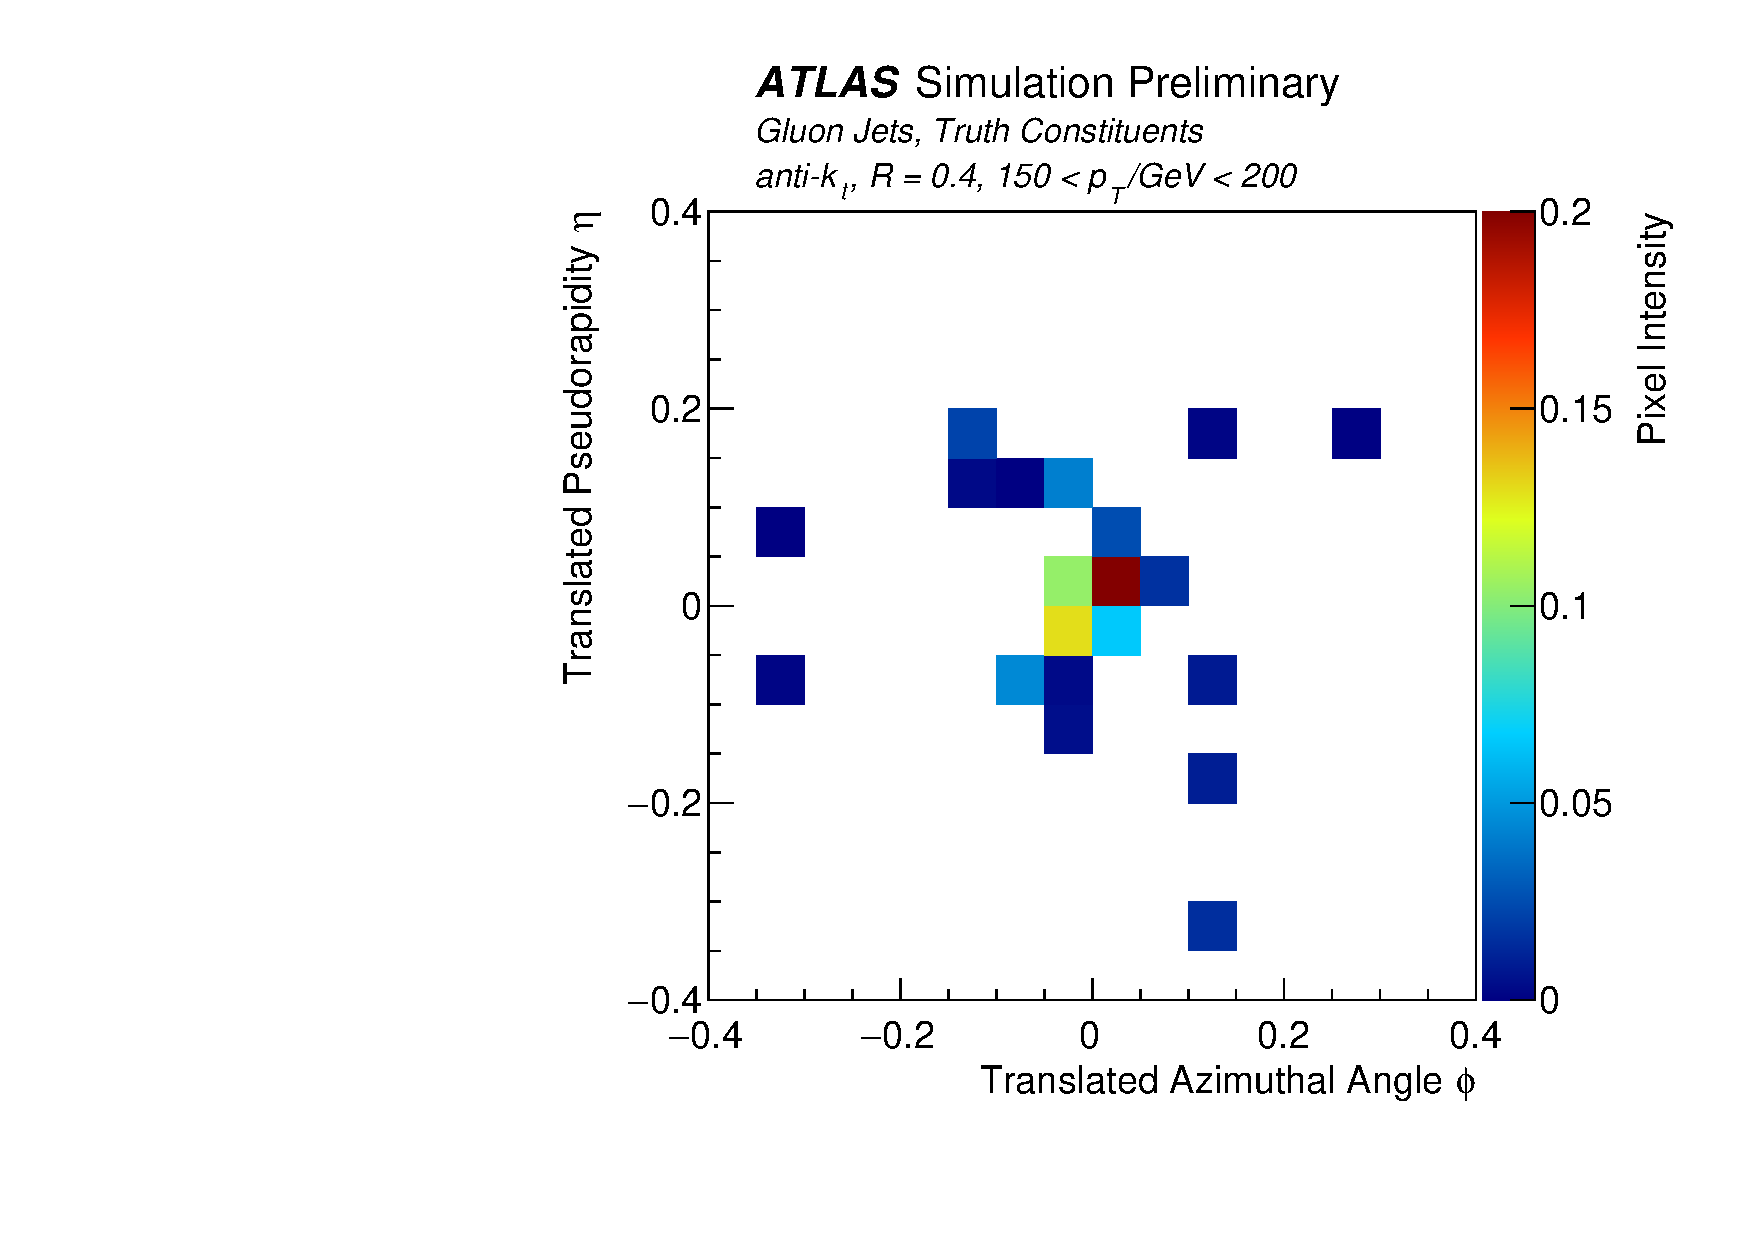
\includegraphics[width=0.45\textwidth]{figures/CNN/gluon_truth_one.pdf}
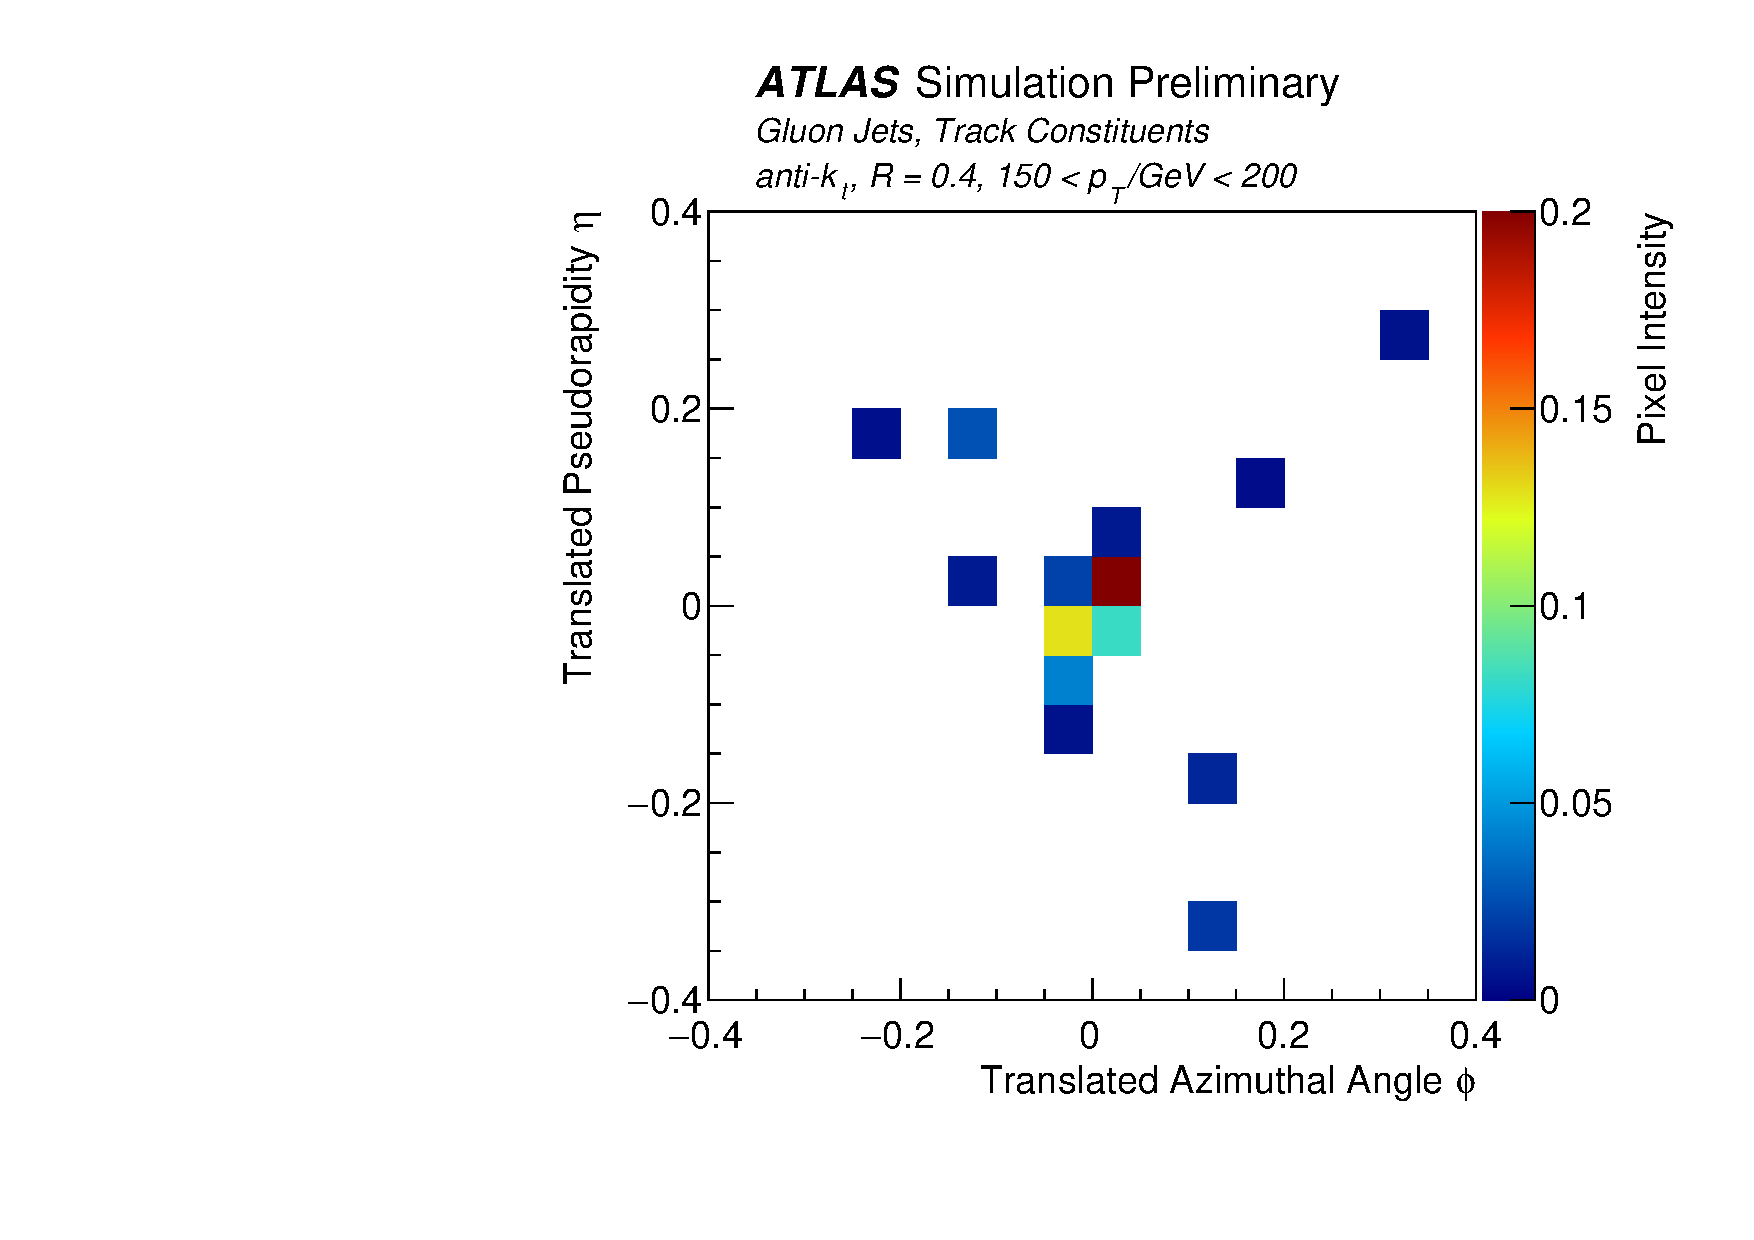
\includegraphics[width=0.45\textwidth]{figures/CNN/gluon_track_one.pdf}\\
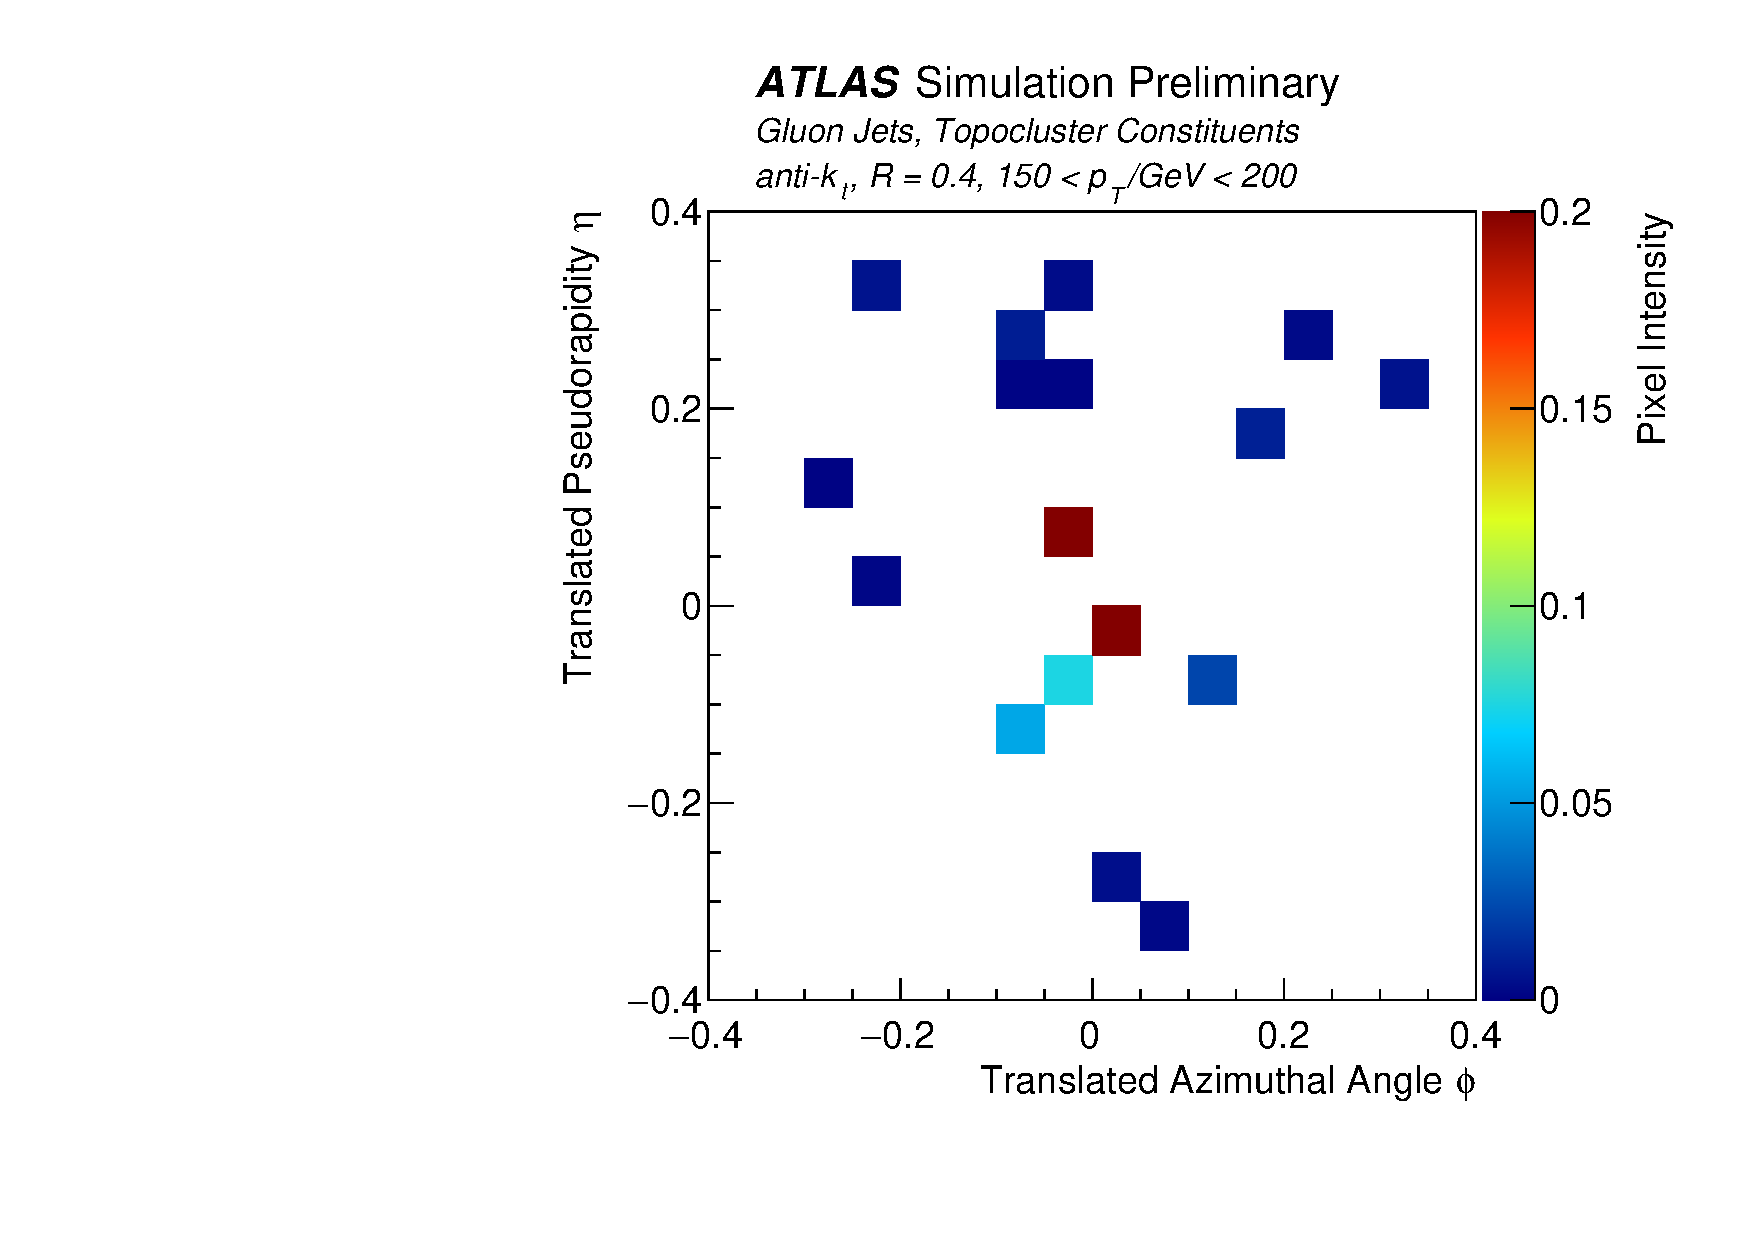
\includegraphics[width=0.45\textwidth]{figures/CNN/gluon_cluster_one.pdf}
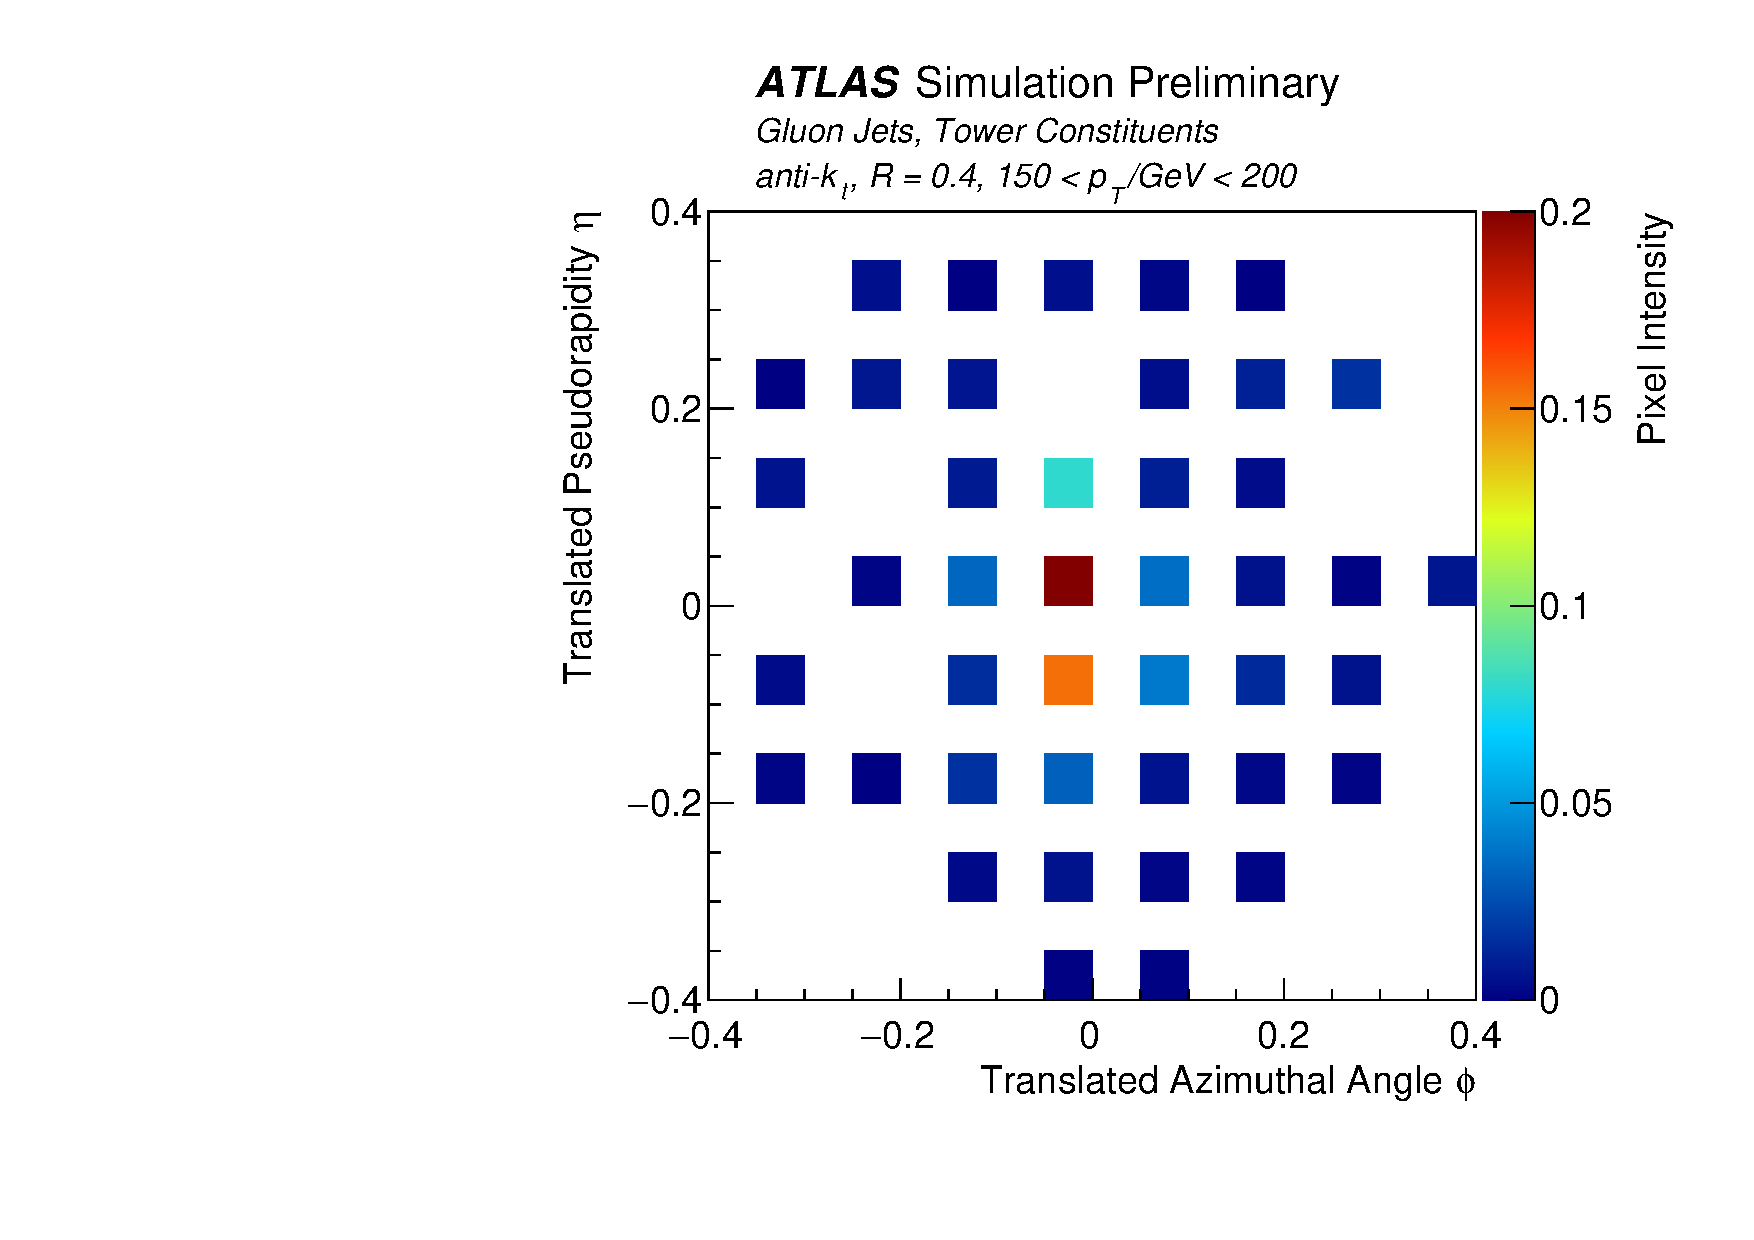
\includegraphics[width=0.45\textwidth]{figures/CNN/gluon_tower_one.pdf}
\caption{The stable particles (top left), track (top right), topocluster (bottom left), and tower (bottom right) images 
for an example gluon jet image.  
The tower image has gaps between hit pixels because the $0.1\times 0.1$ towers are projected onto a $0.05\times 0.05$ jet image.}
\label{fig:cnn-oneimage}
\end{center}
\end{figure}

\begin{figure}[h!]
\begin{center}
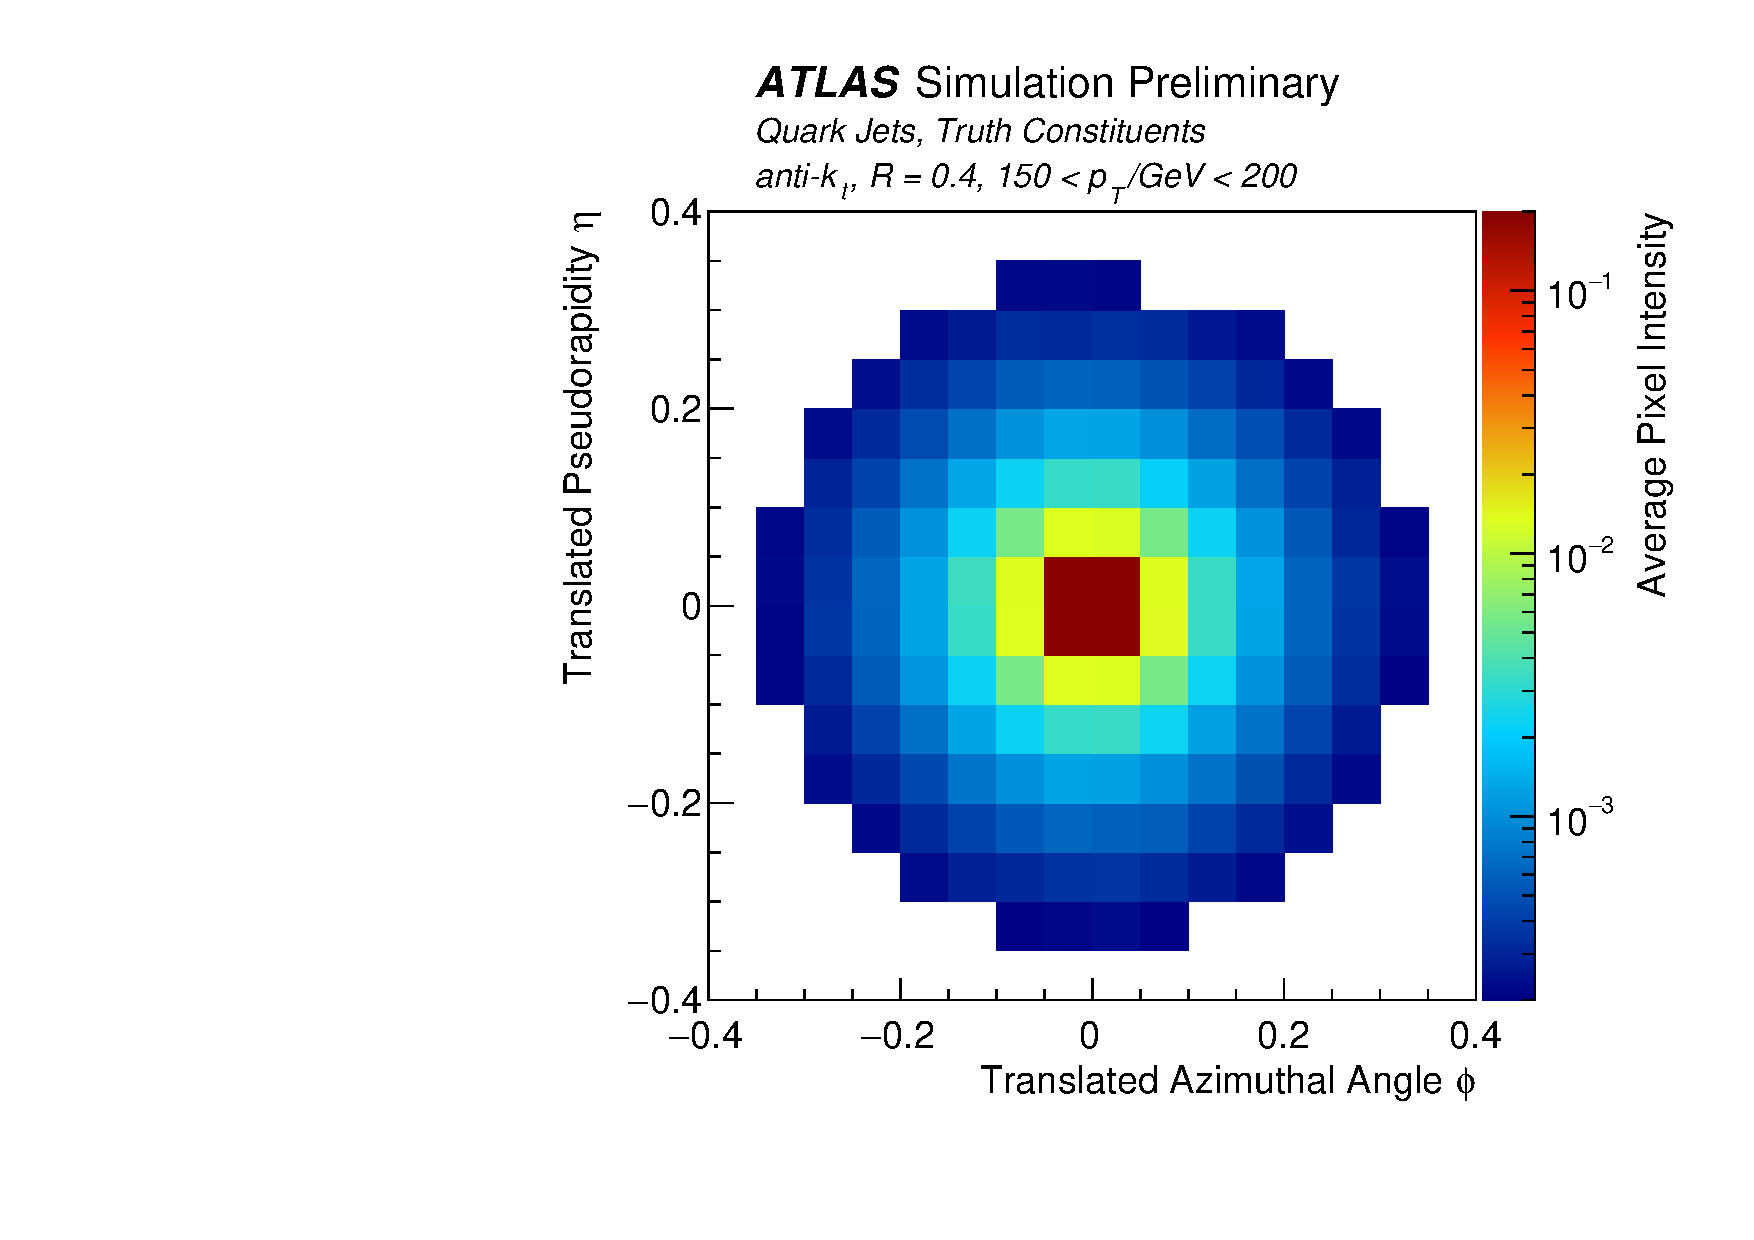
\includegraphics[width=0.31\textwidth]{figures/CNN/quark_truth.pdf}
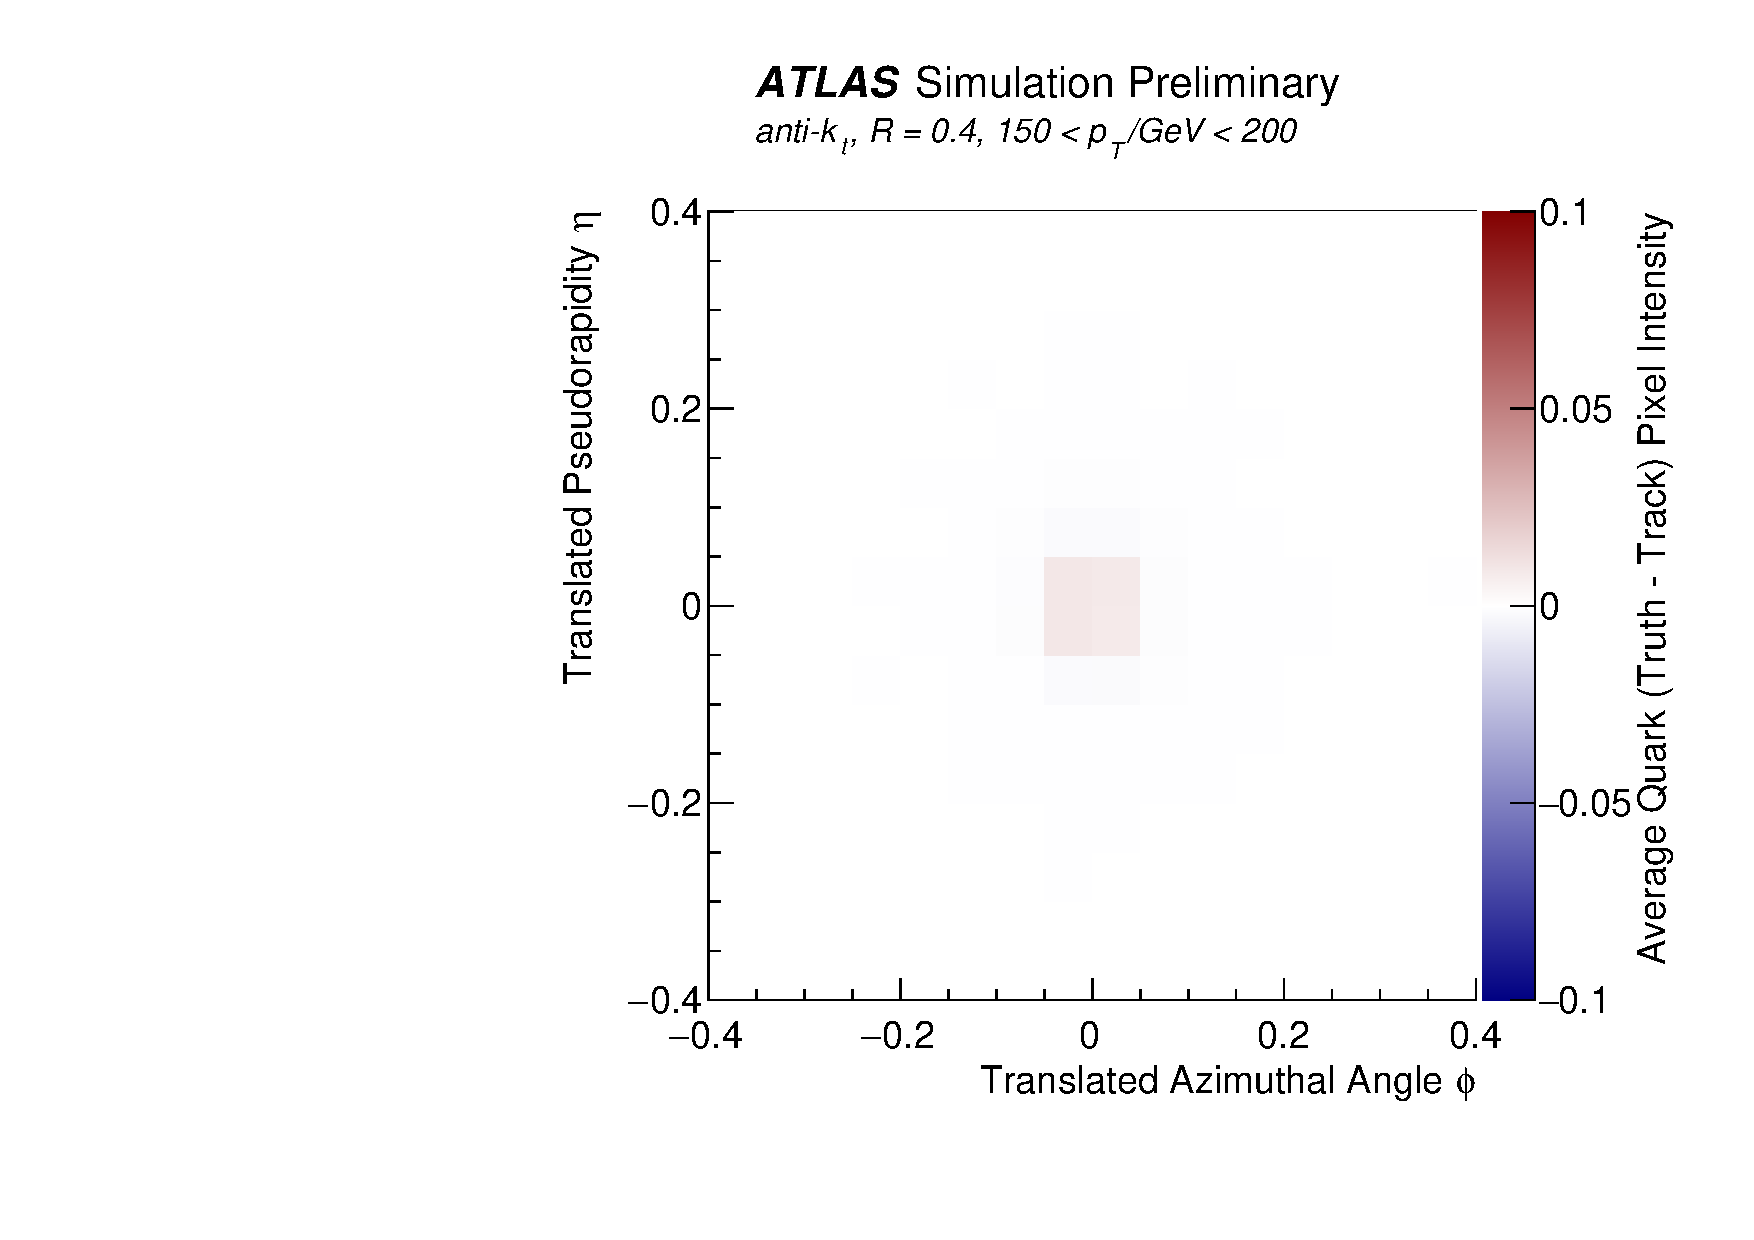
\includegraphics[width=0.31\textwidth]{figures/CNN/diff_quark_truth_track.pdf}
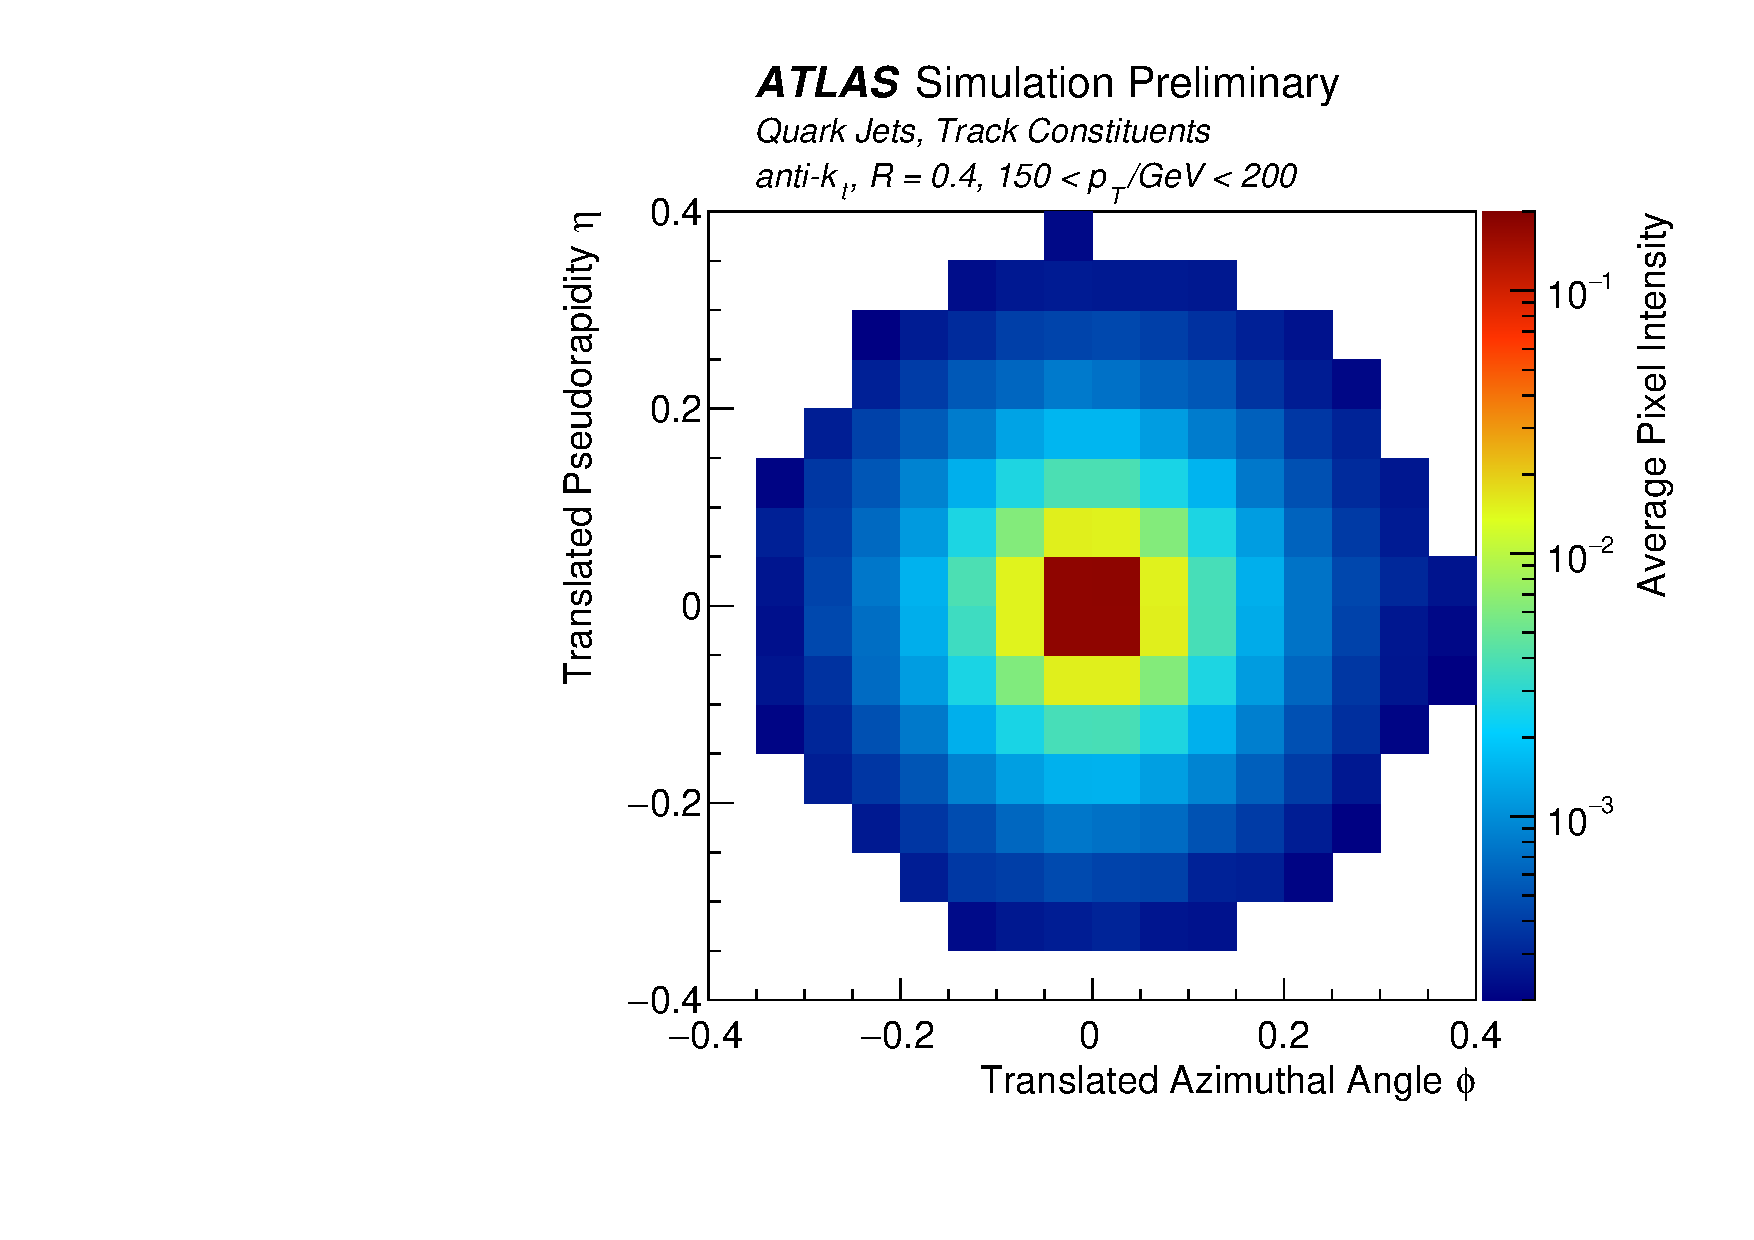
\includegraphics[width=0.31\textwidth]{figures/CNN/quark_track.pdf}\\
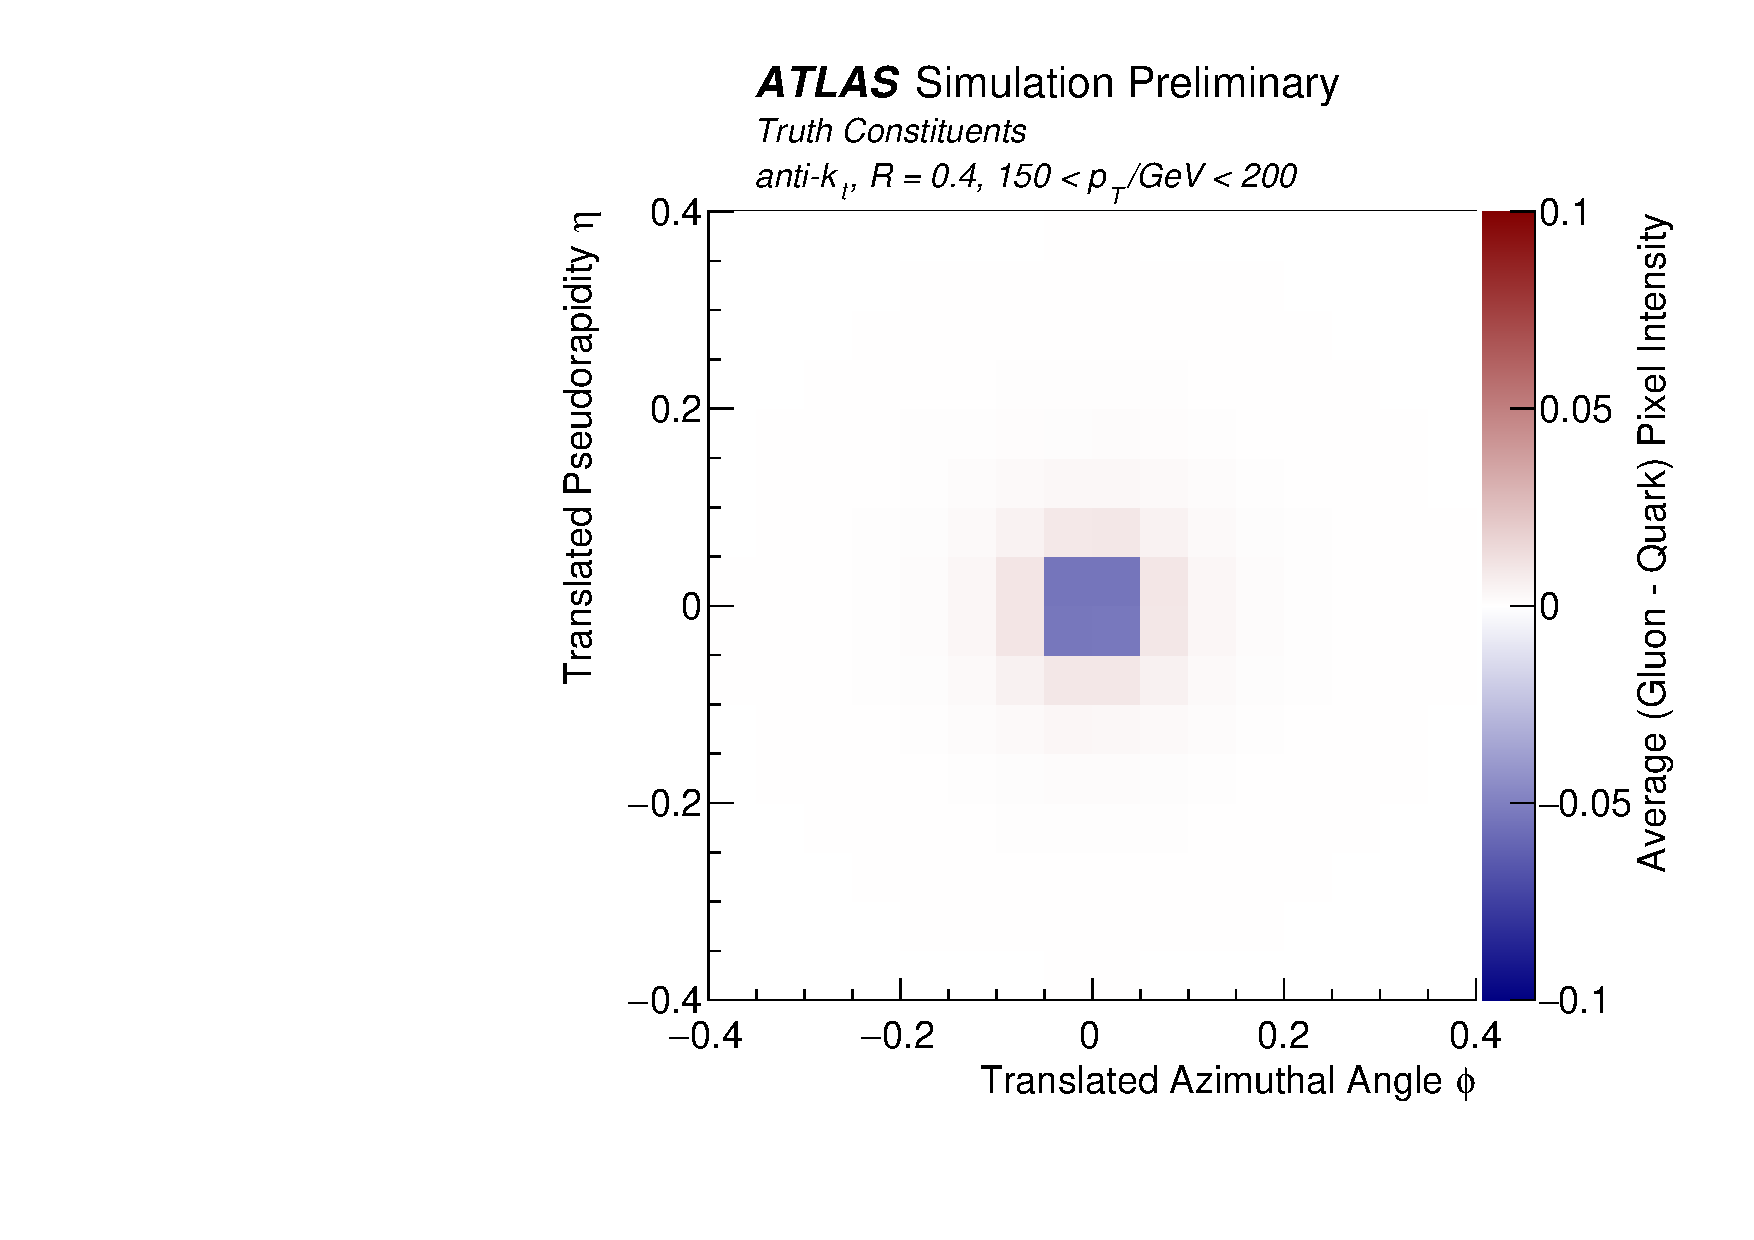
\includegraphics[width=0.31\textwidth]{figures/CNN/diff_truth.pdf}\hspace{54mm}
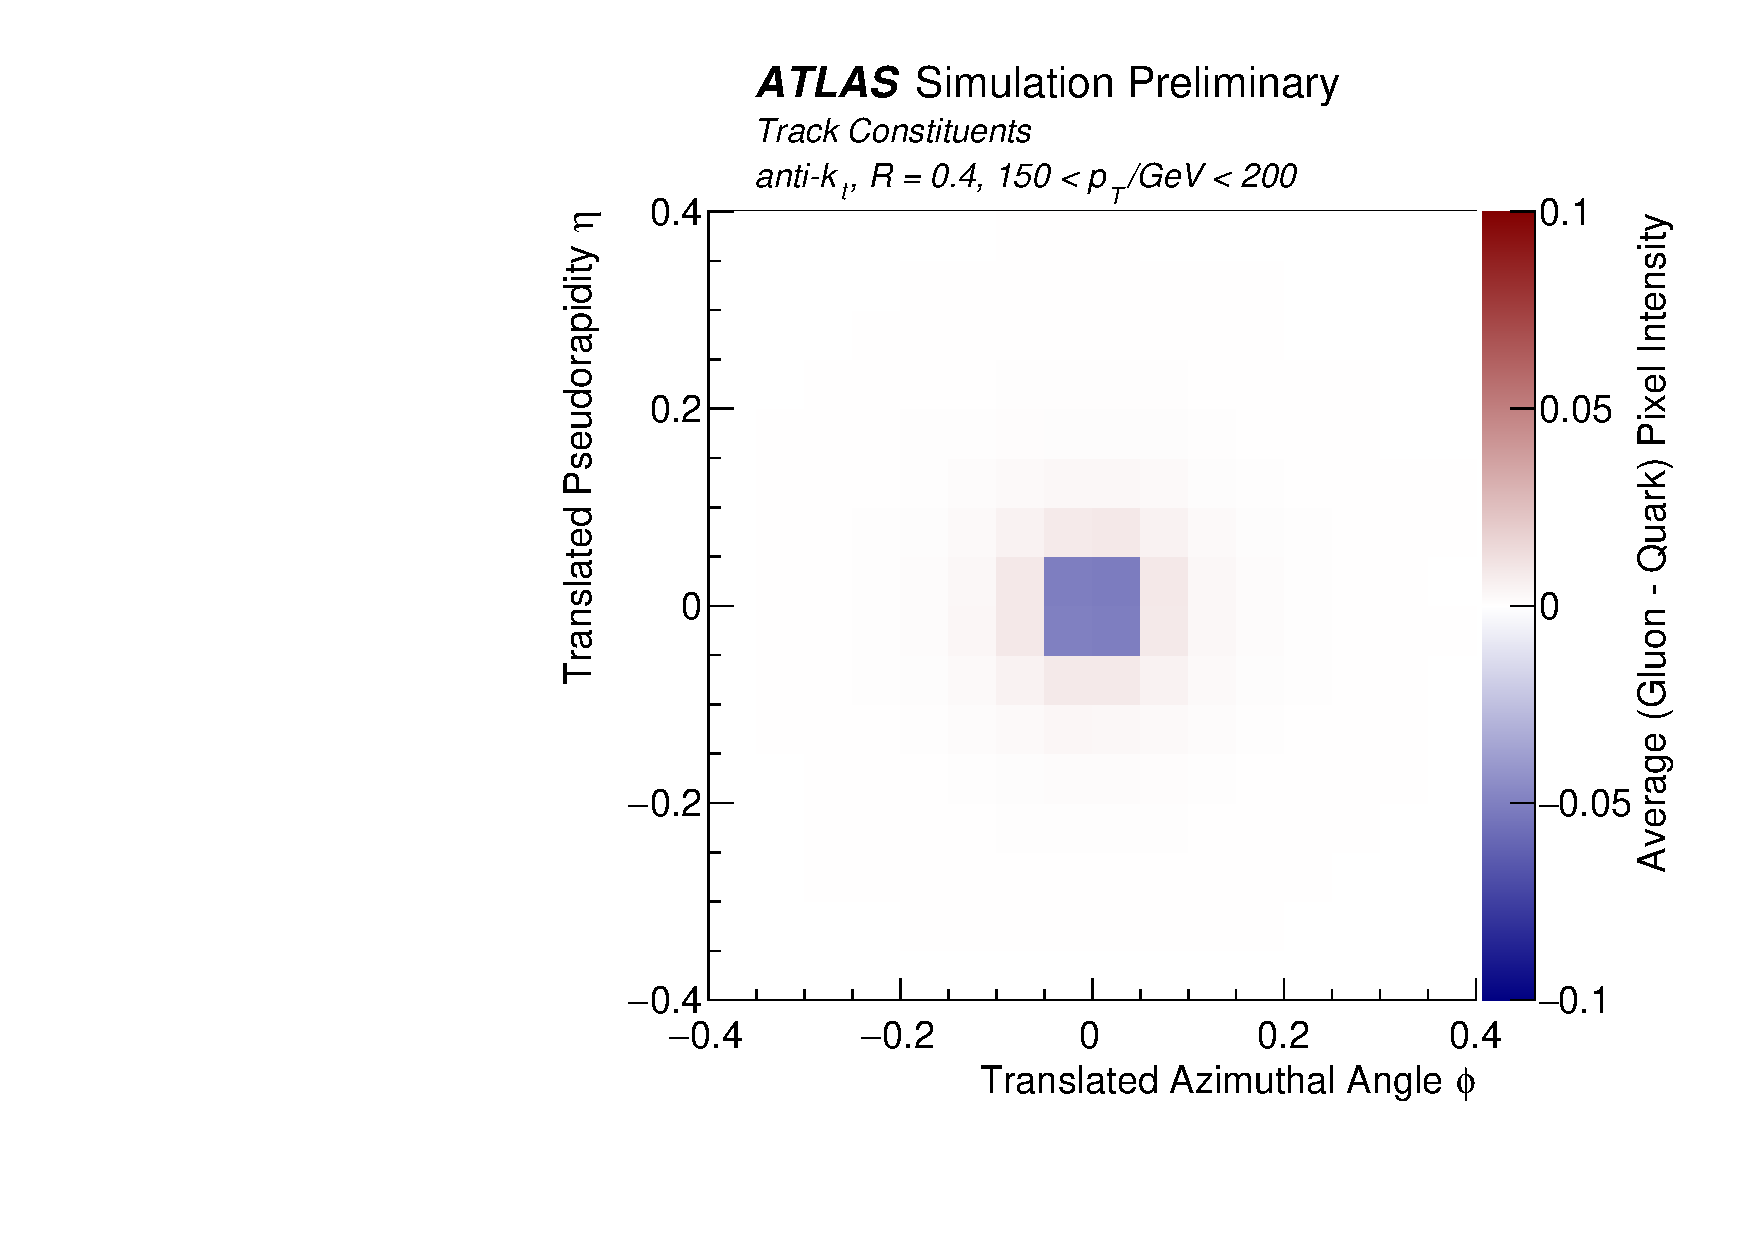
\includegraphics[width=0.31\textwidth]{figures/CNN/diff_track.pdf}\\
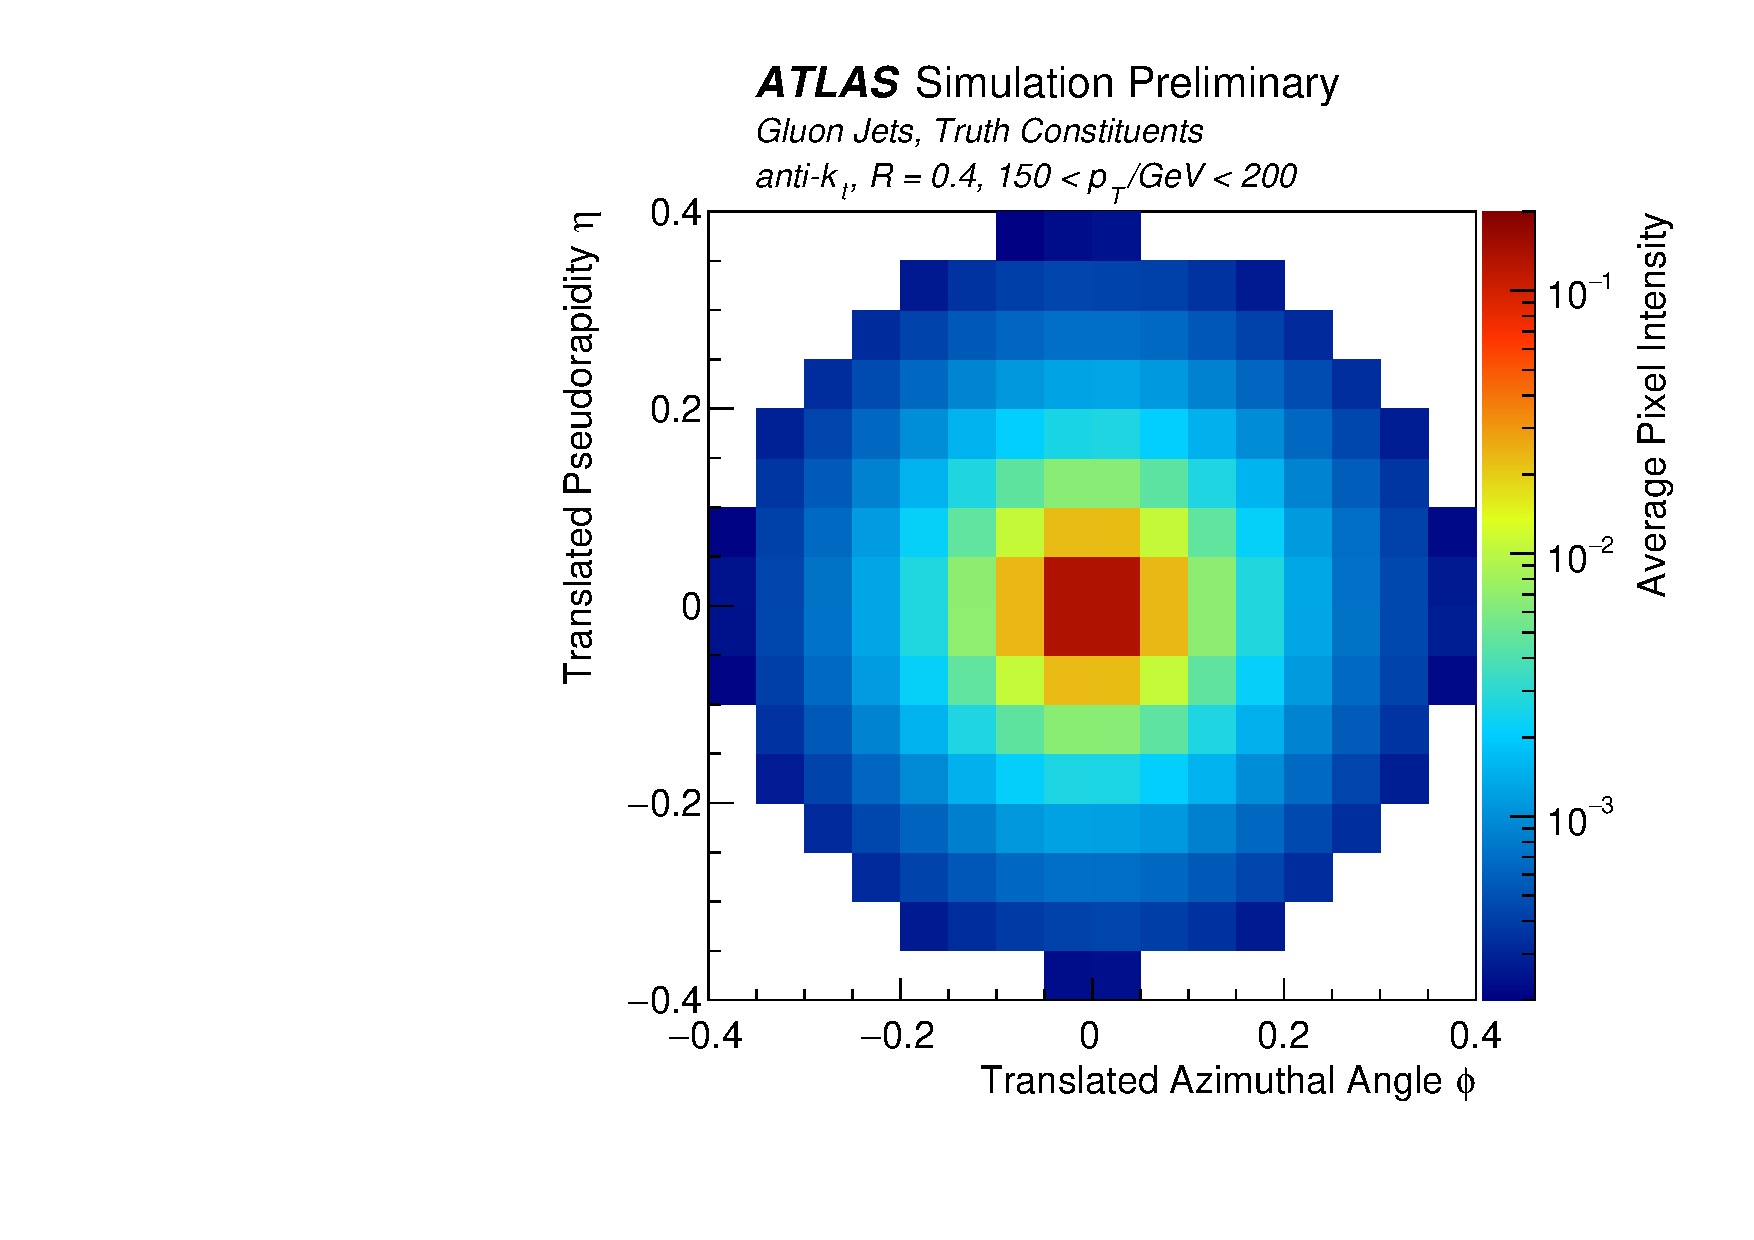
\includegraphics[width=0.31\textwidth]{figures/CNN/gluon_truth.pdf}
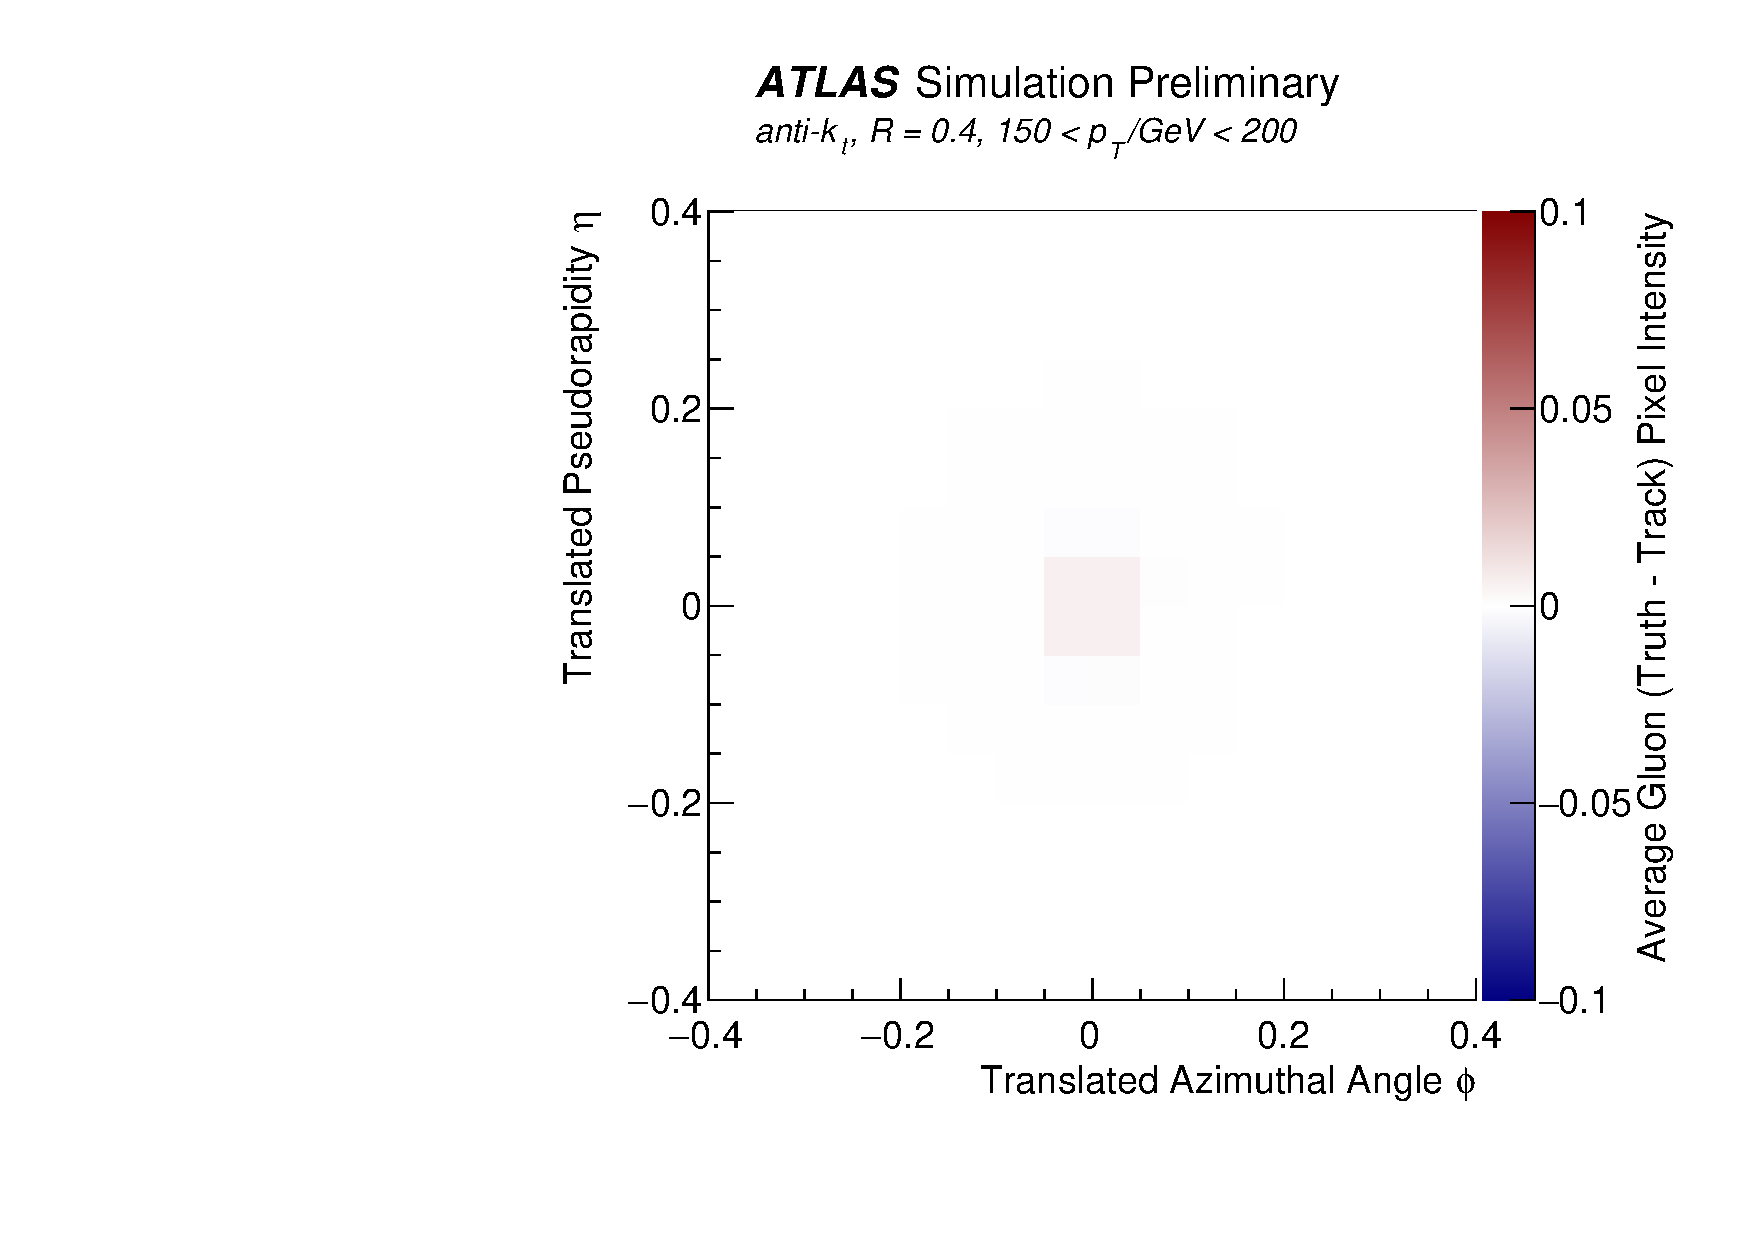
\includegraphics[width=0.31\textwidth]{figures/CNN/diff_gluon_truth_track.pdf}
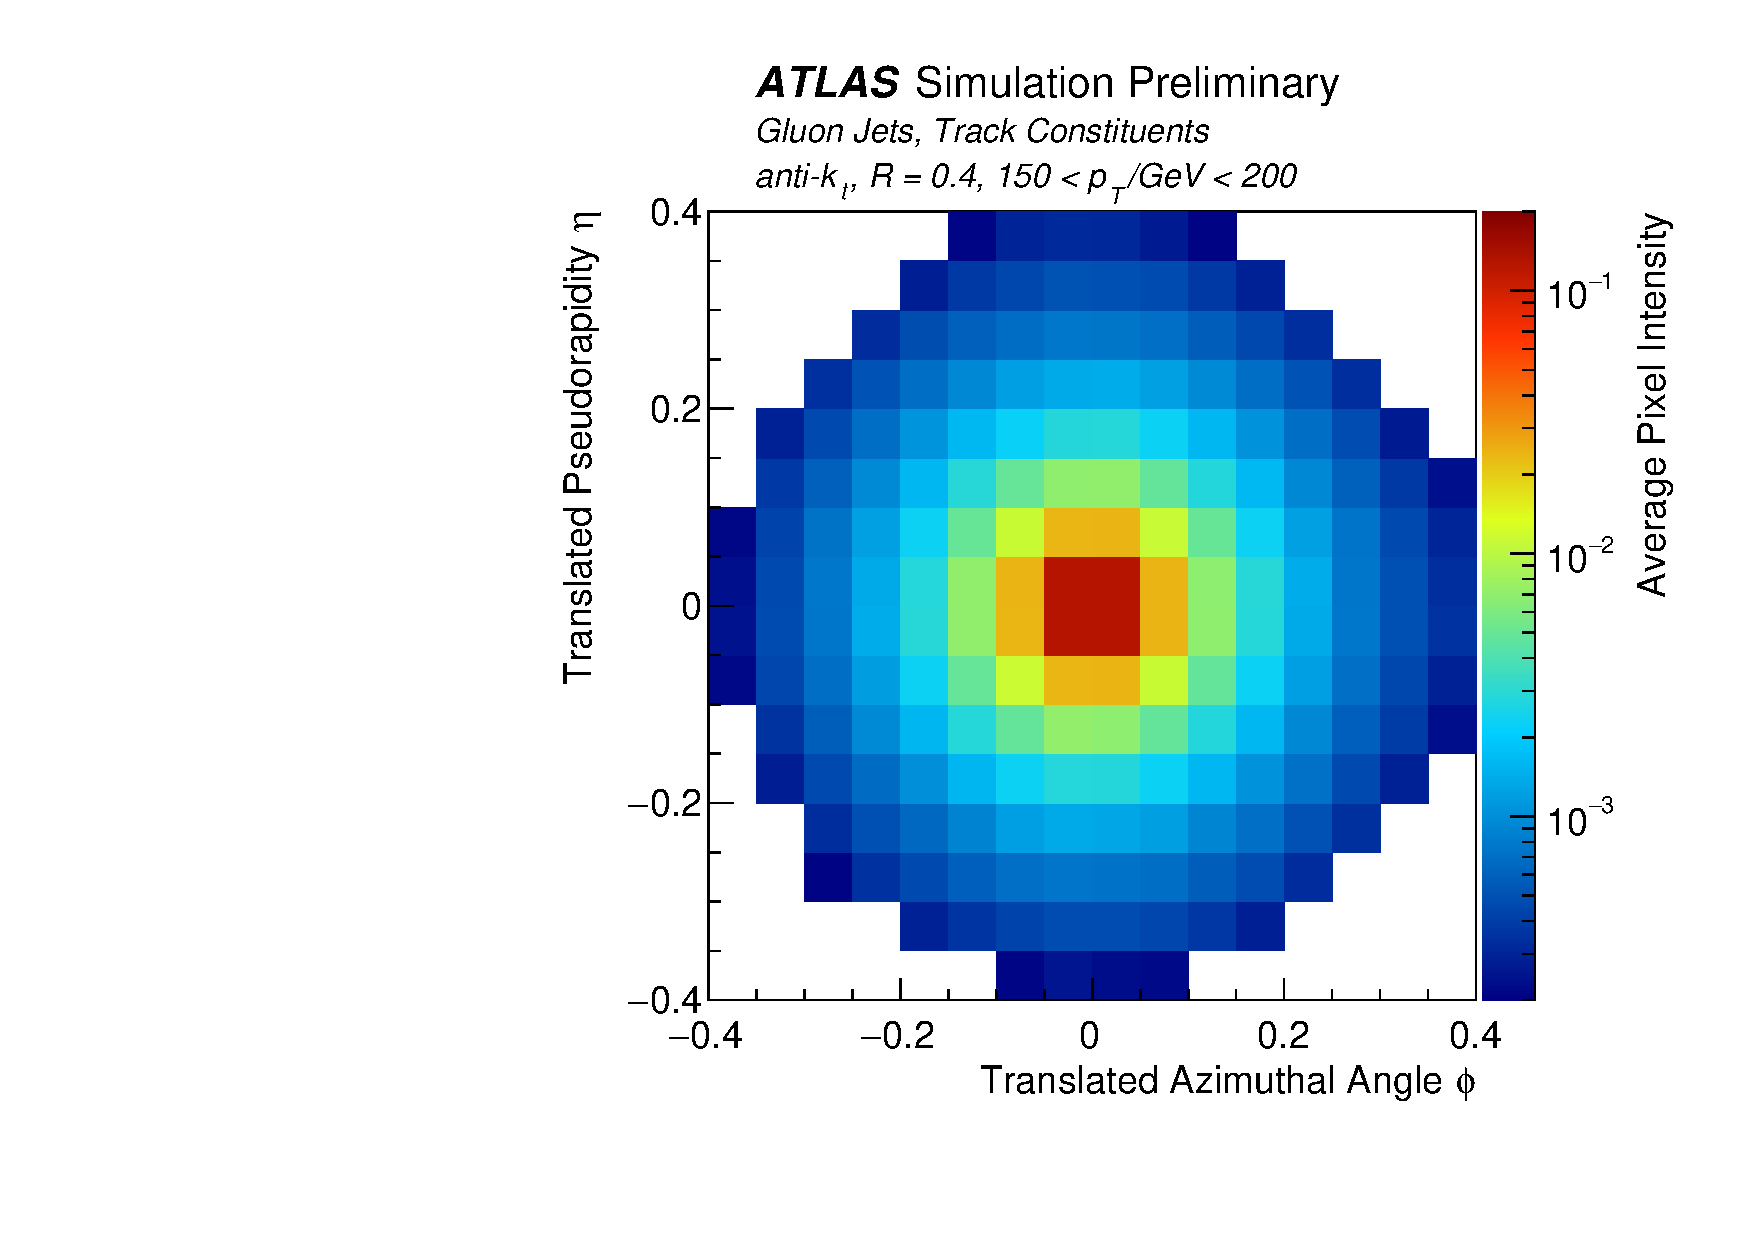
\includegraphics[width=0.31\textwidth]{figures/CNN/gluon_track.pdf}
\caption{The four corners show the average quark (upper) and gluon (lower) jet images, from true constituents, both charged and neutral, (left) and reconstructed tracks (right); the four plots on the edges show the difference between the adjacent plots, for example the top plot shows the difference between the average quark jet for stable particles and reconstructed tracks. Quark-jets are more collimated than gluon ones, and track images show slightly less central activity than in the true jet.}
\label{fig:cnn-avg:truthtrack}
\end{center}
\end{figure}

\begin{figure}[h!]
\begin{center}
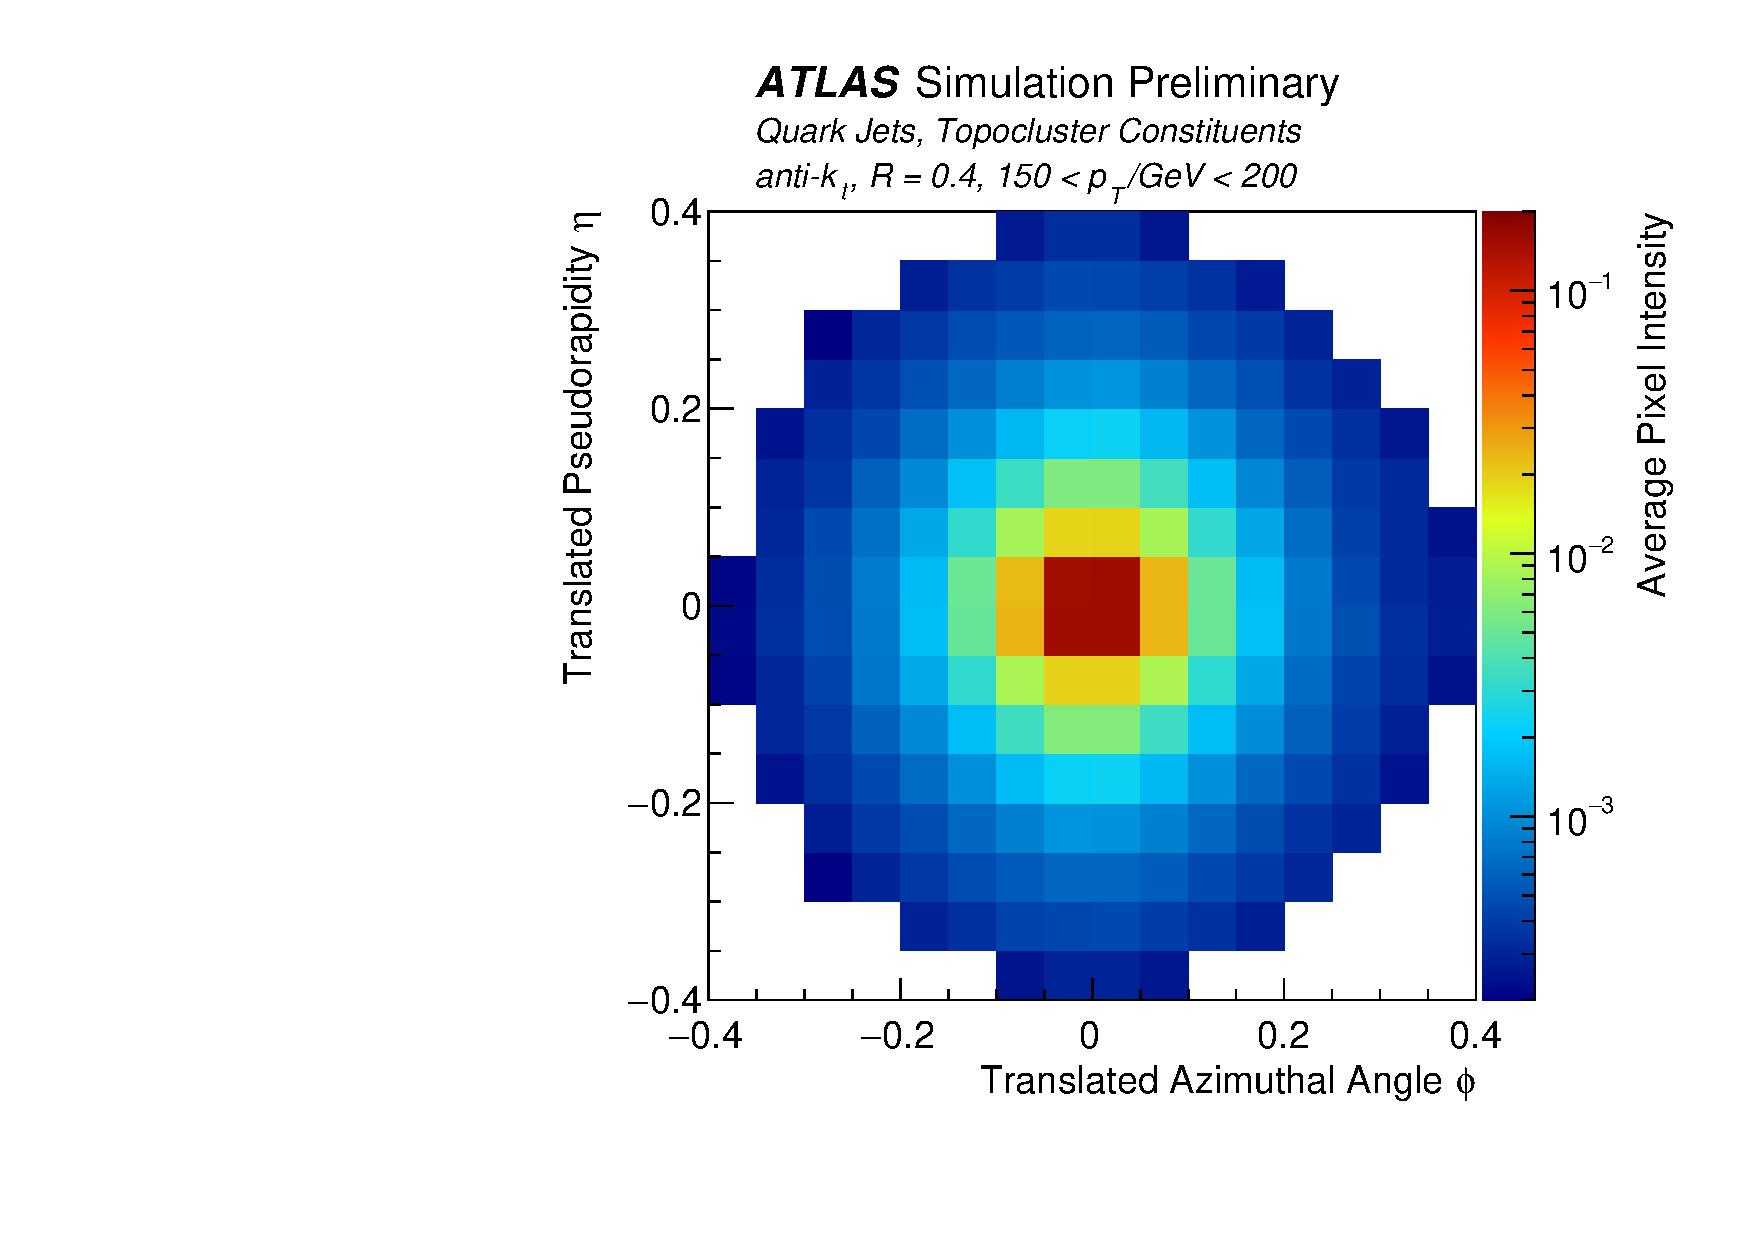
\includegraphics[width=0.31\textwidth]{figures/CNN/quark_cluster.pdf}
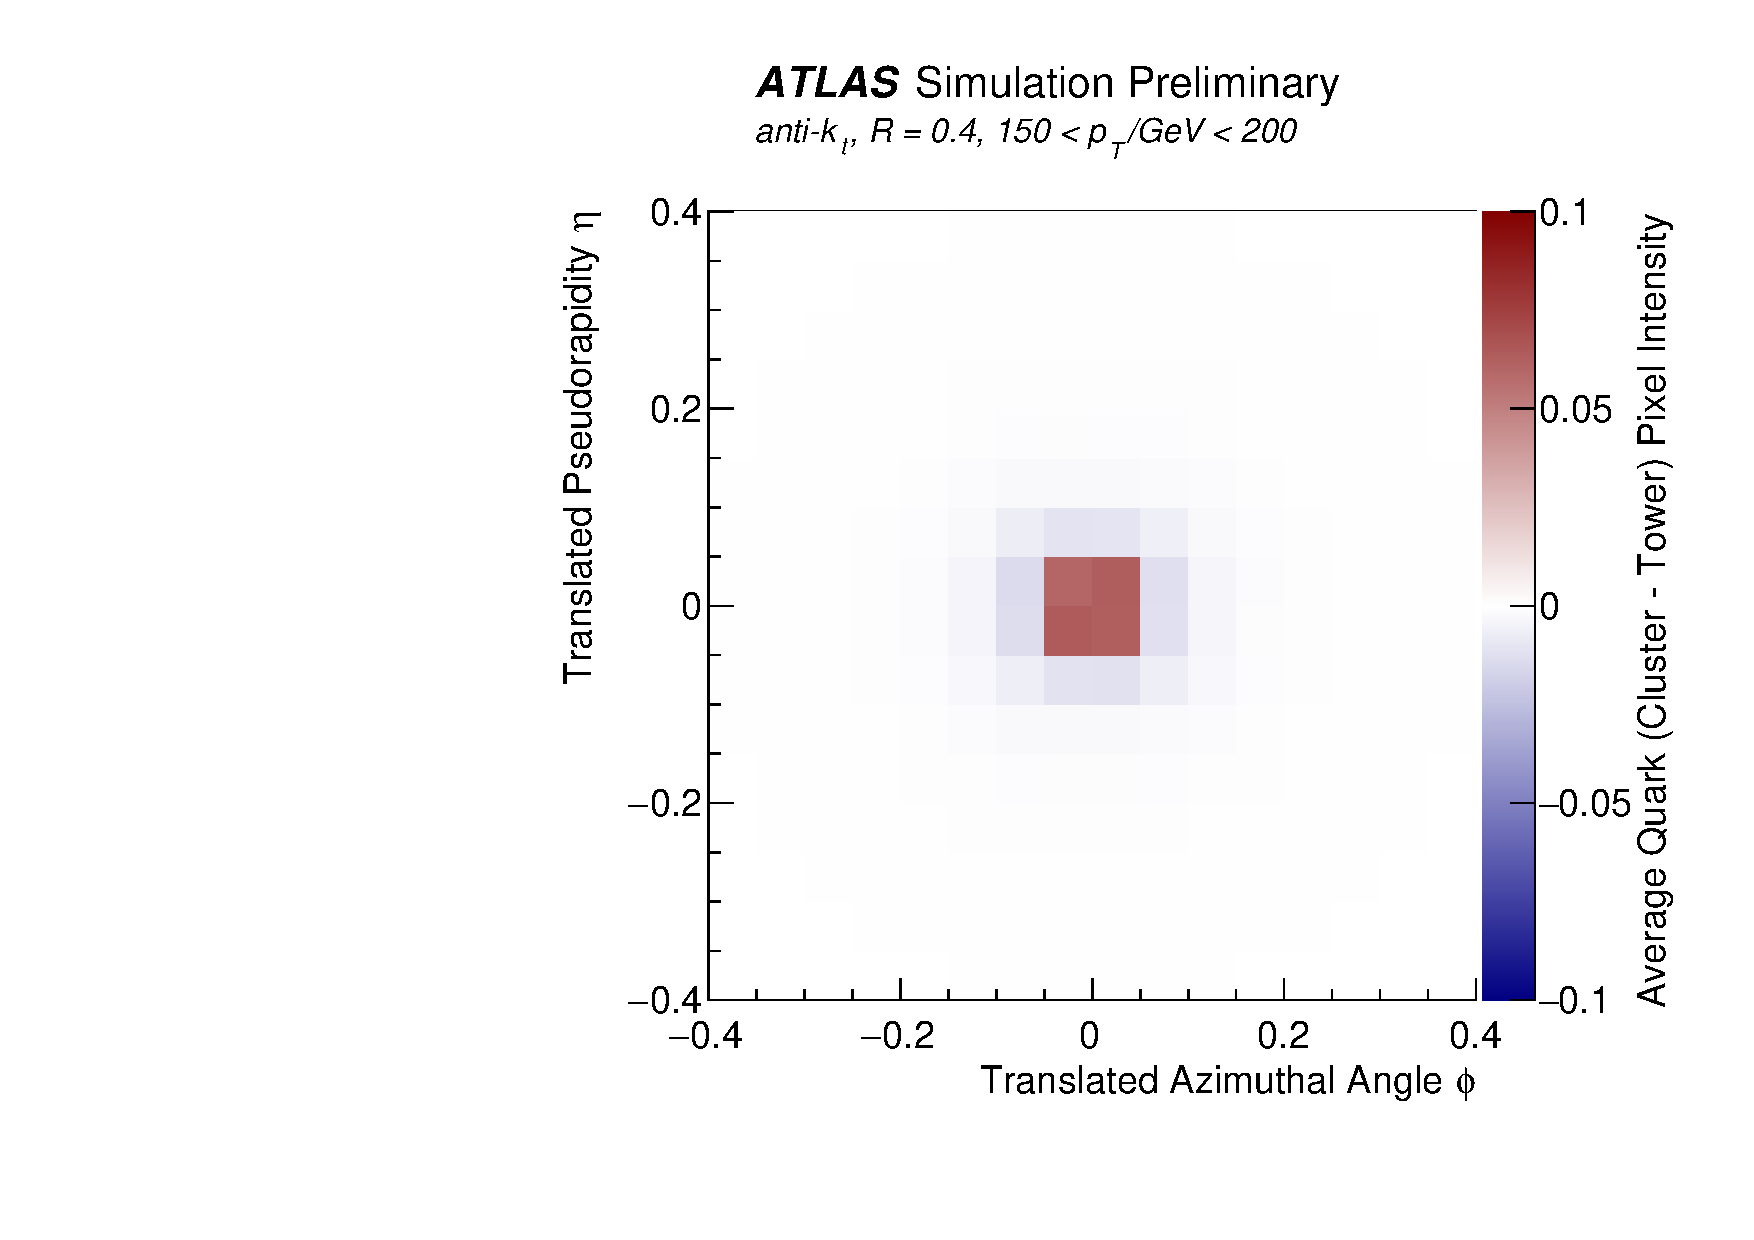
\includegraphics[width=0.31\textwidth]{figures/CNN/diff_quark_cluster_tower.pdf}
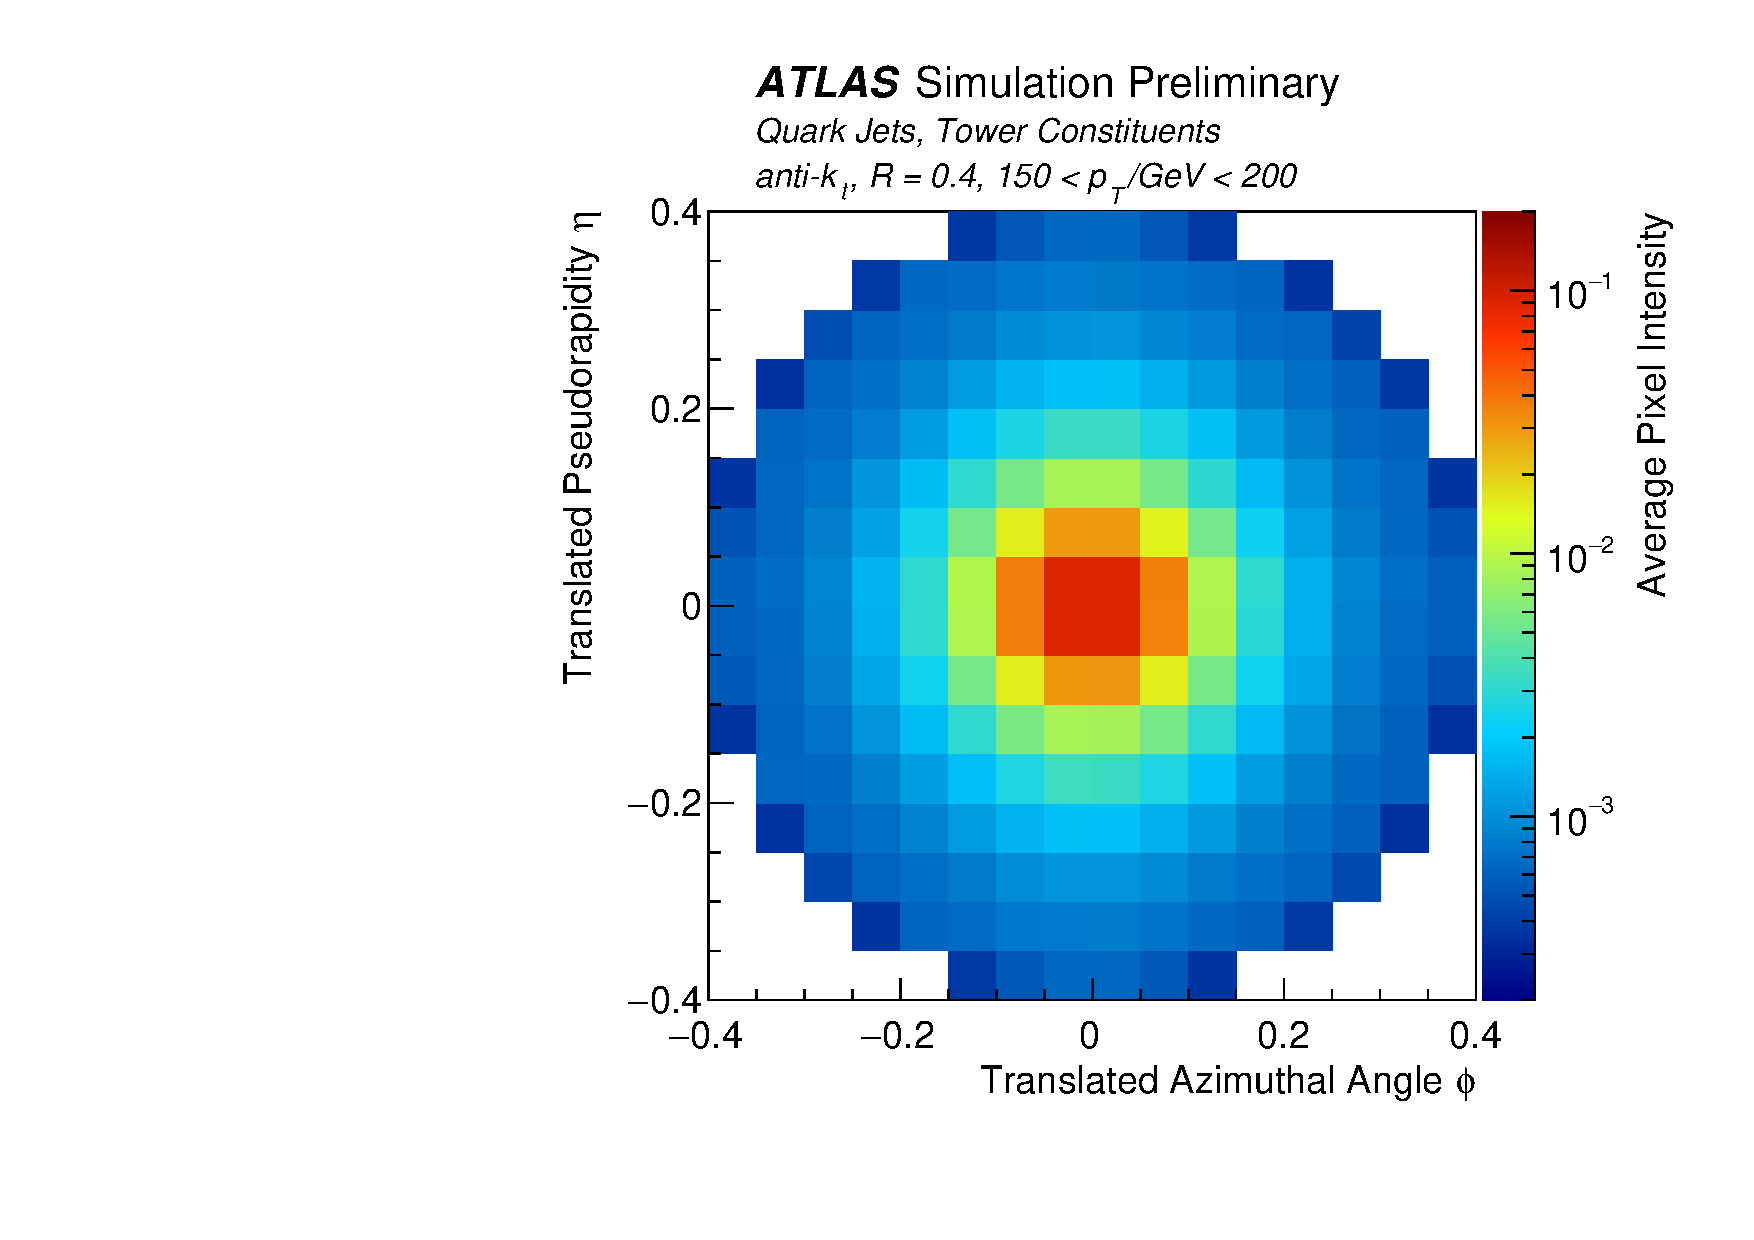
\includegraphics[width=0.31\textwidth]{figures/CNN/quark_tower.pdf}\\
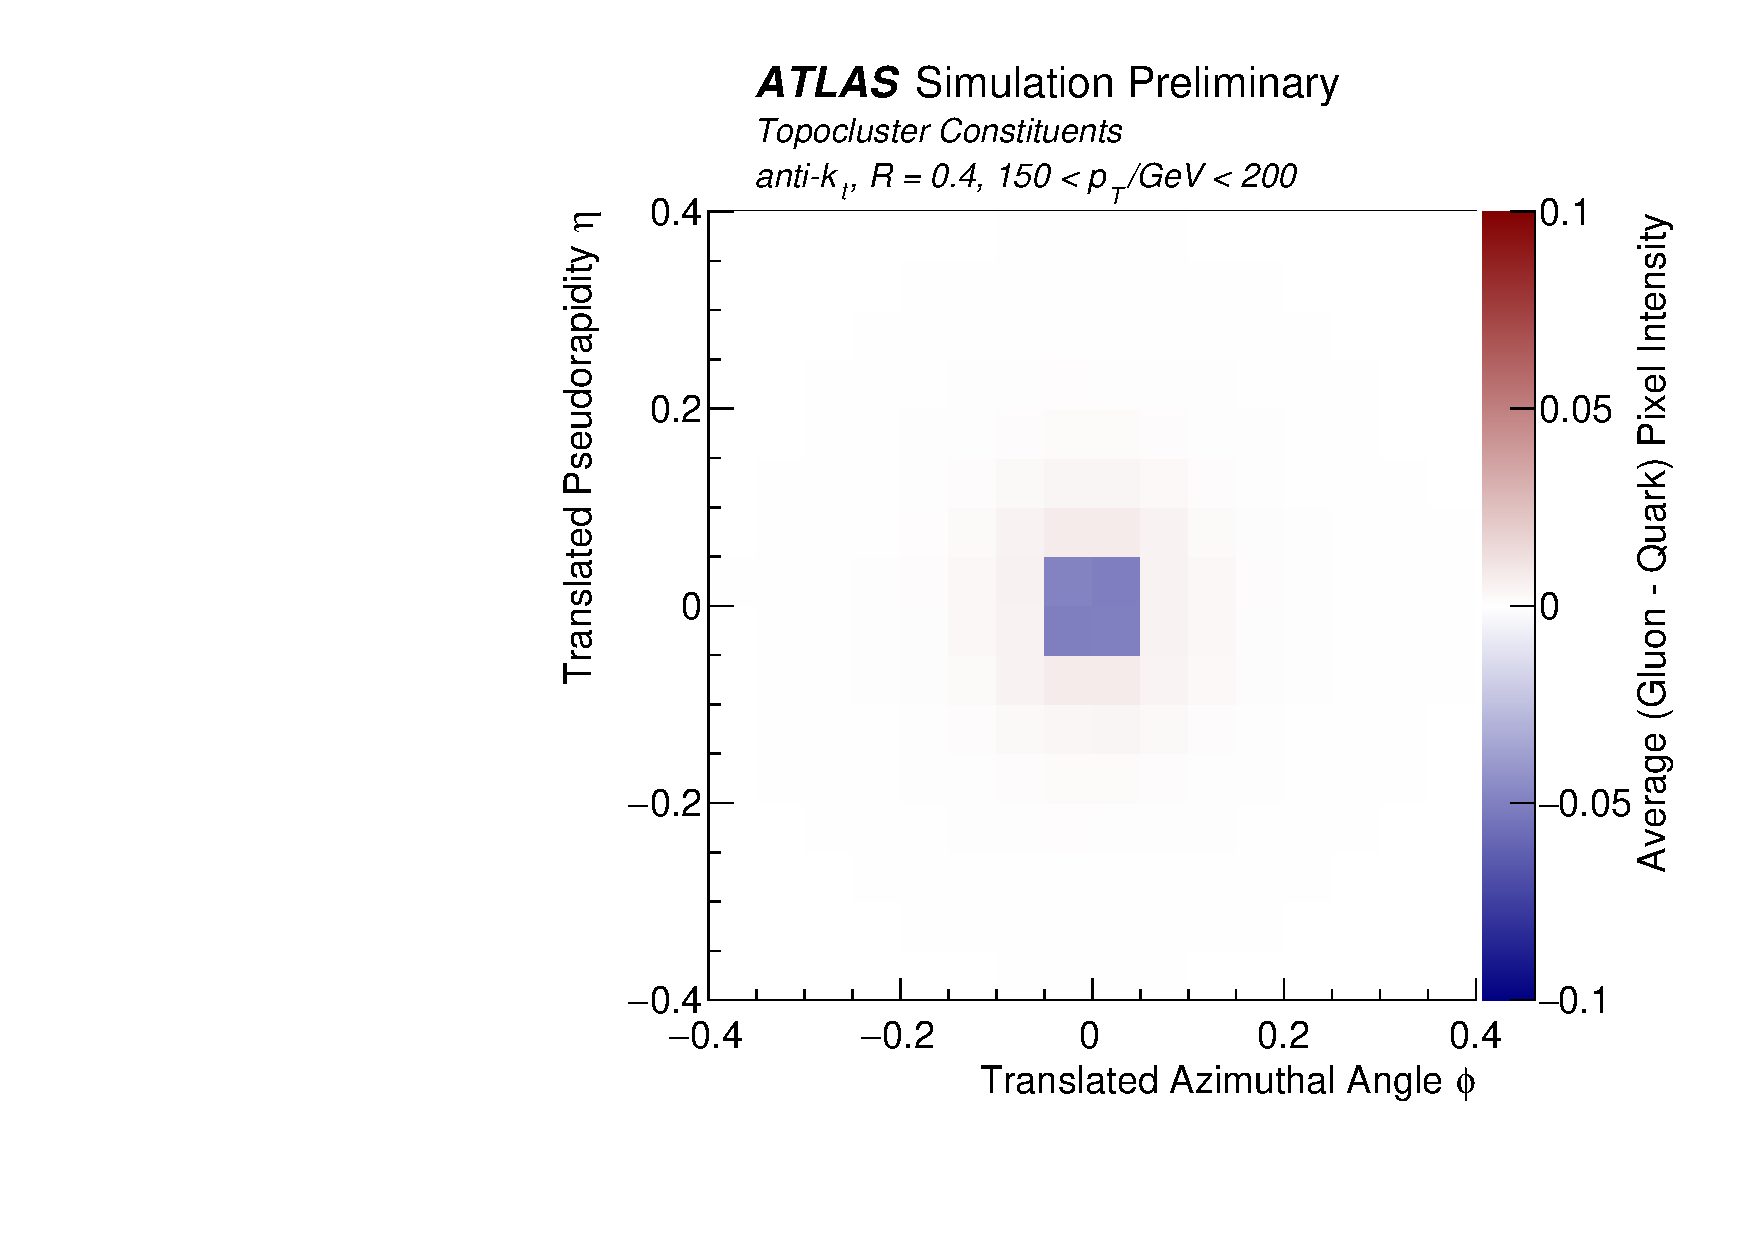
\includegraphics[width=0.31\textwidth]{figures/CNN/diff_cluster.pdf}\hspace{54mm}
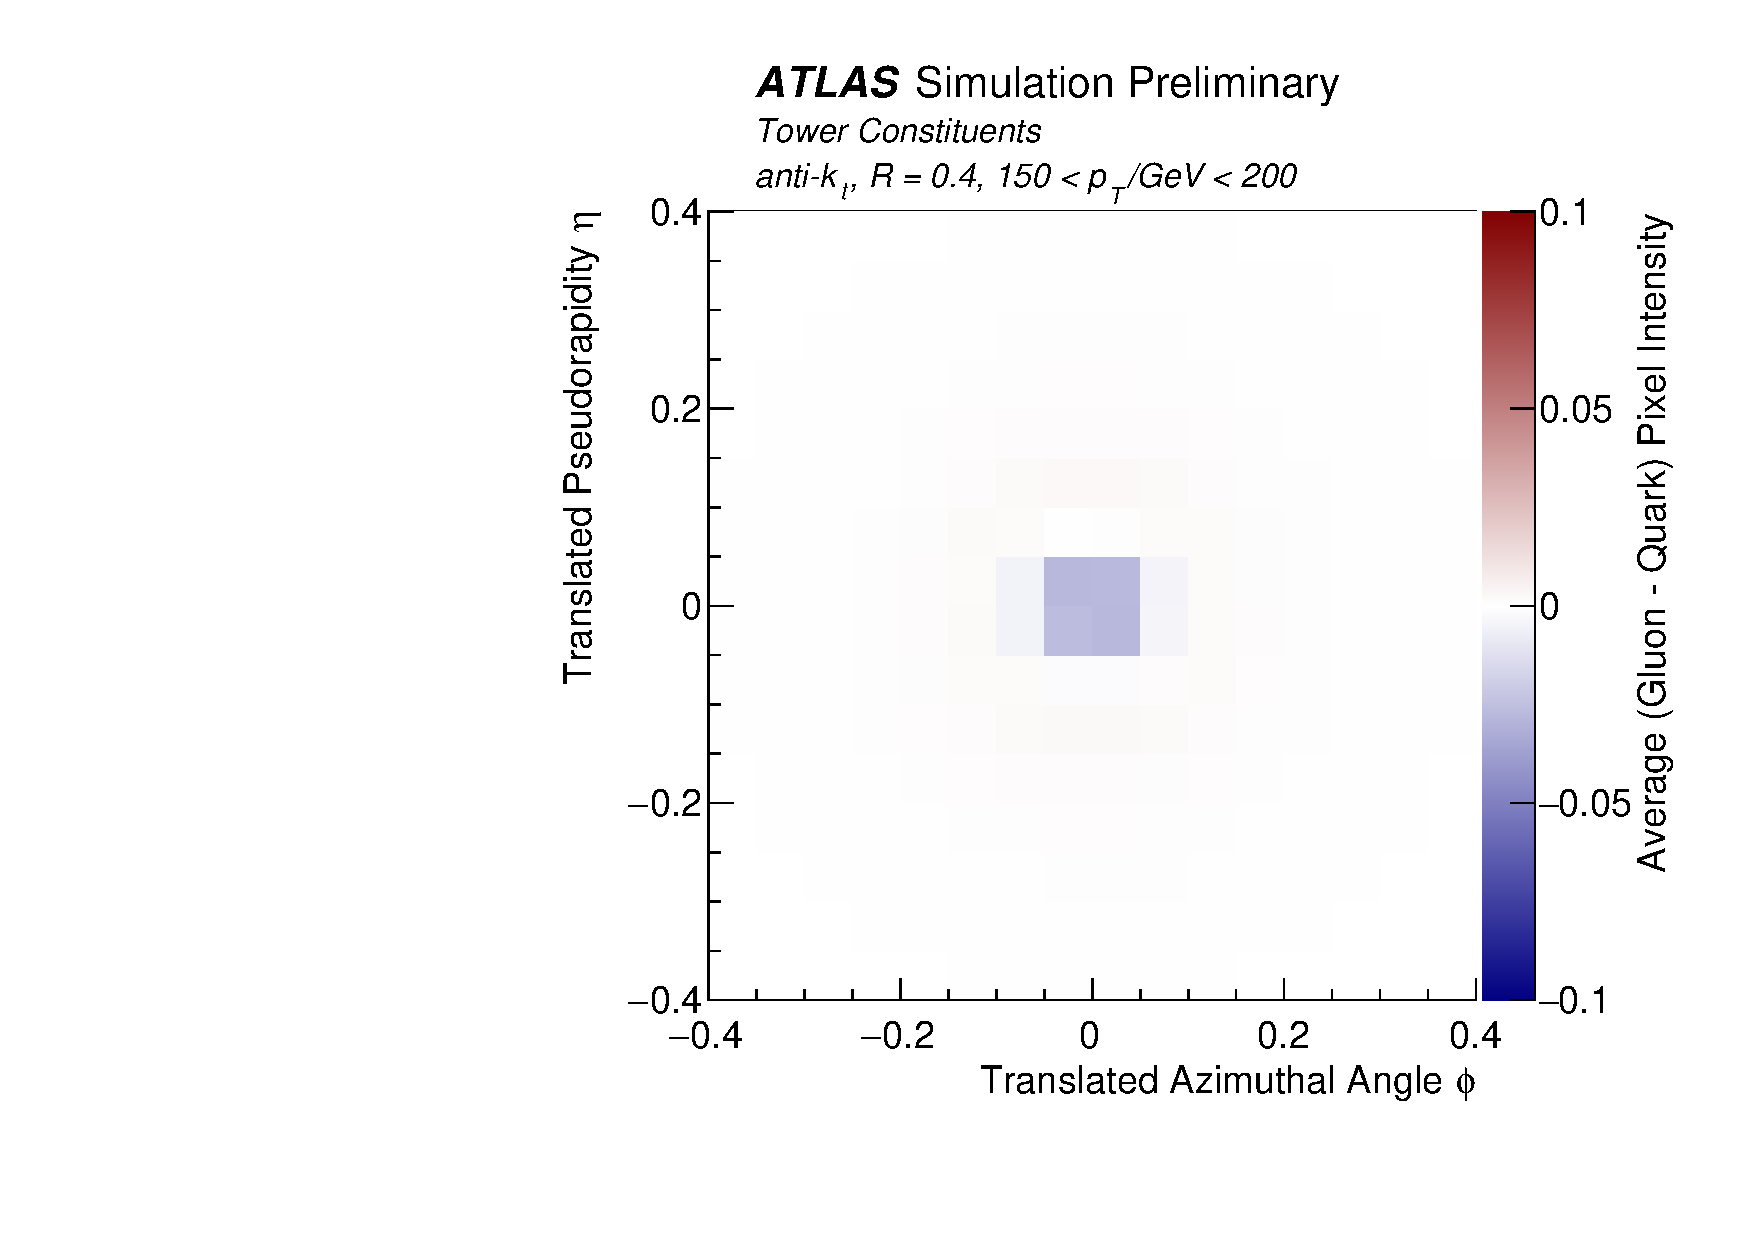
\includegraphics[width=0.31\textwidth]{figures/CNN/diff_tower.pdf}\\
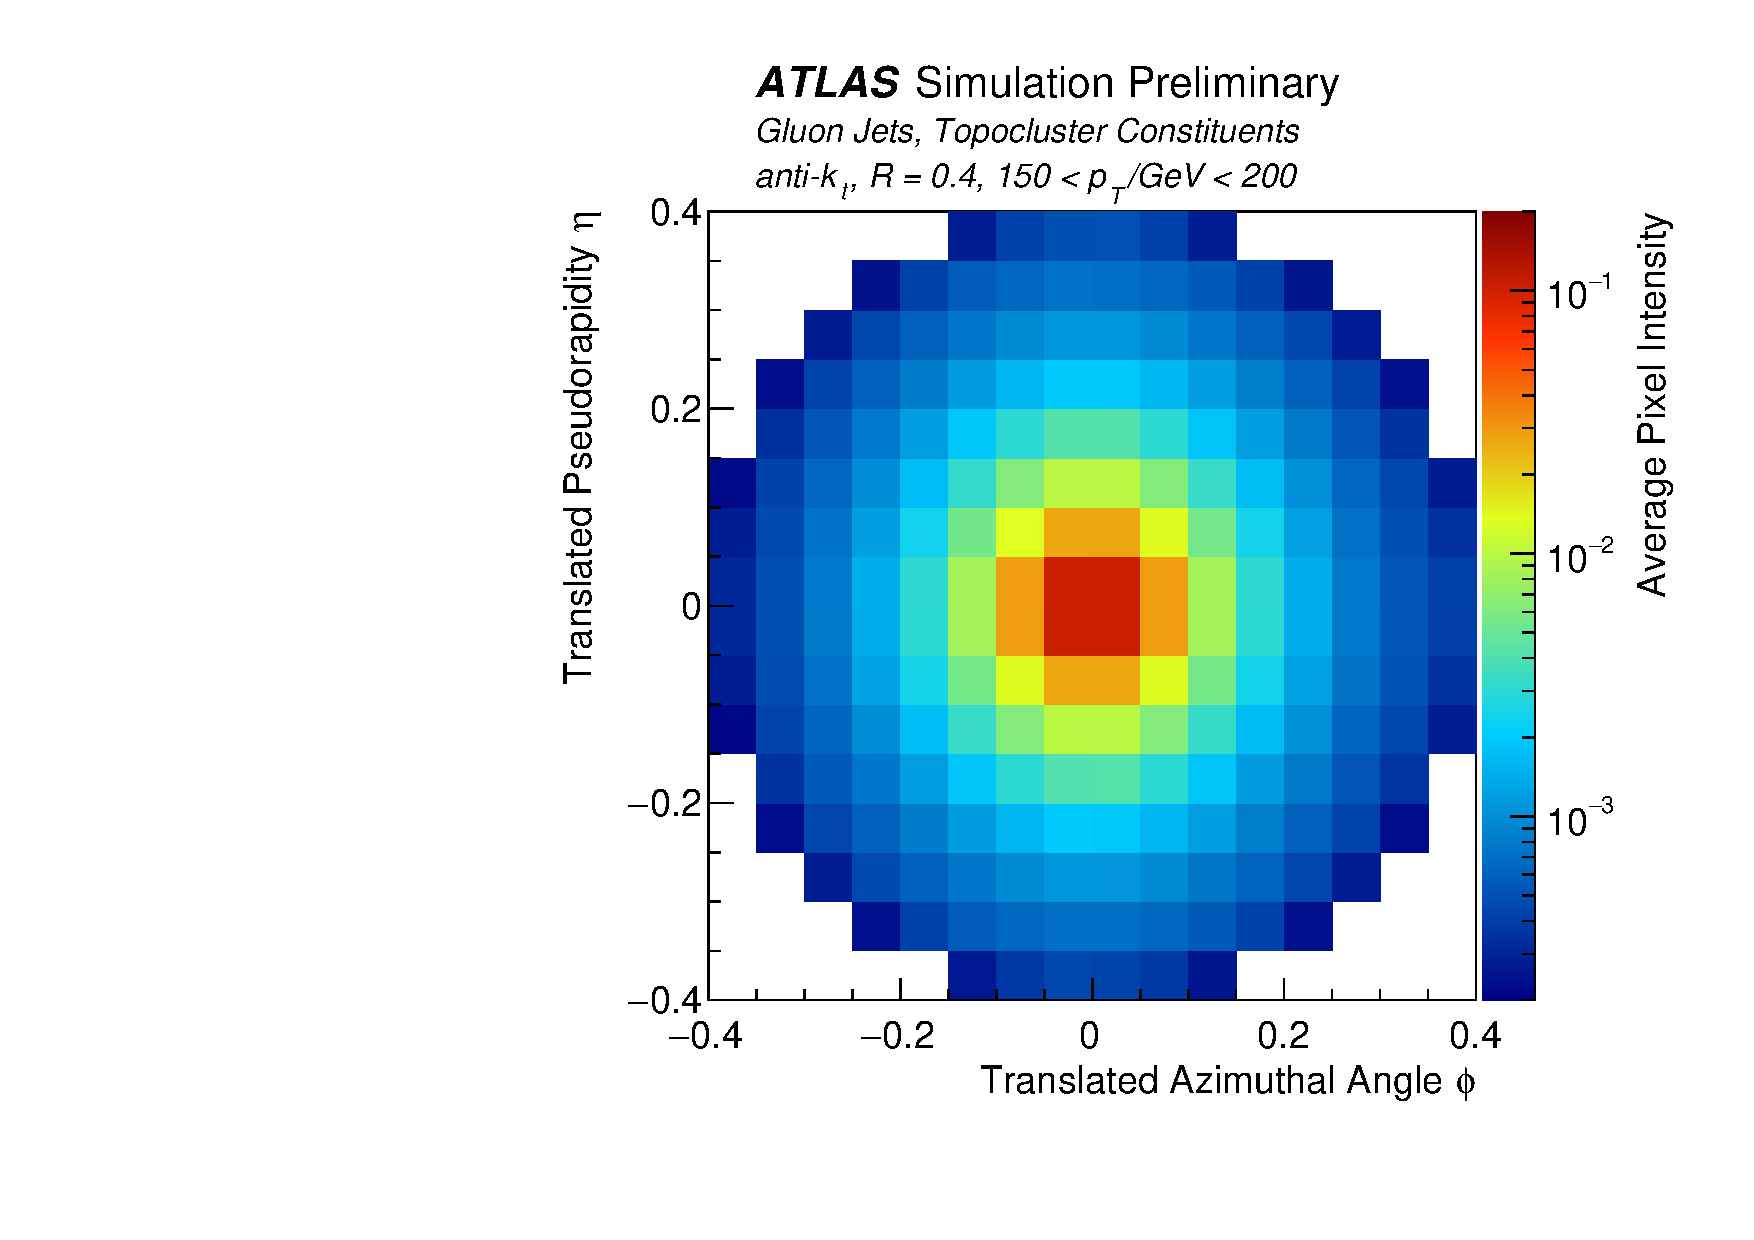
\includegraphics[width=0.31\textwidth]{figures/CNN/gluon_cluster.pdf}
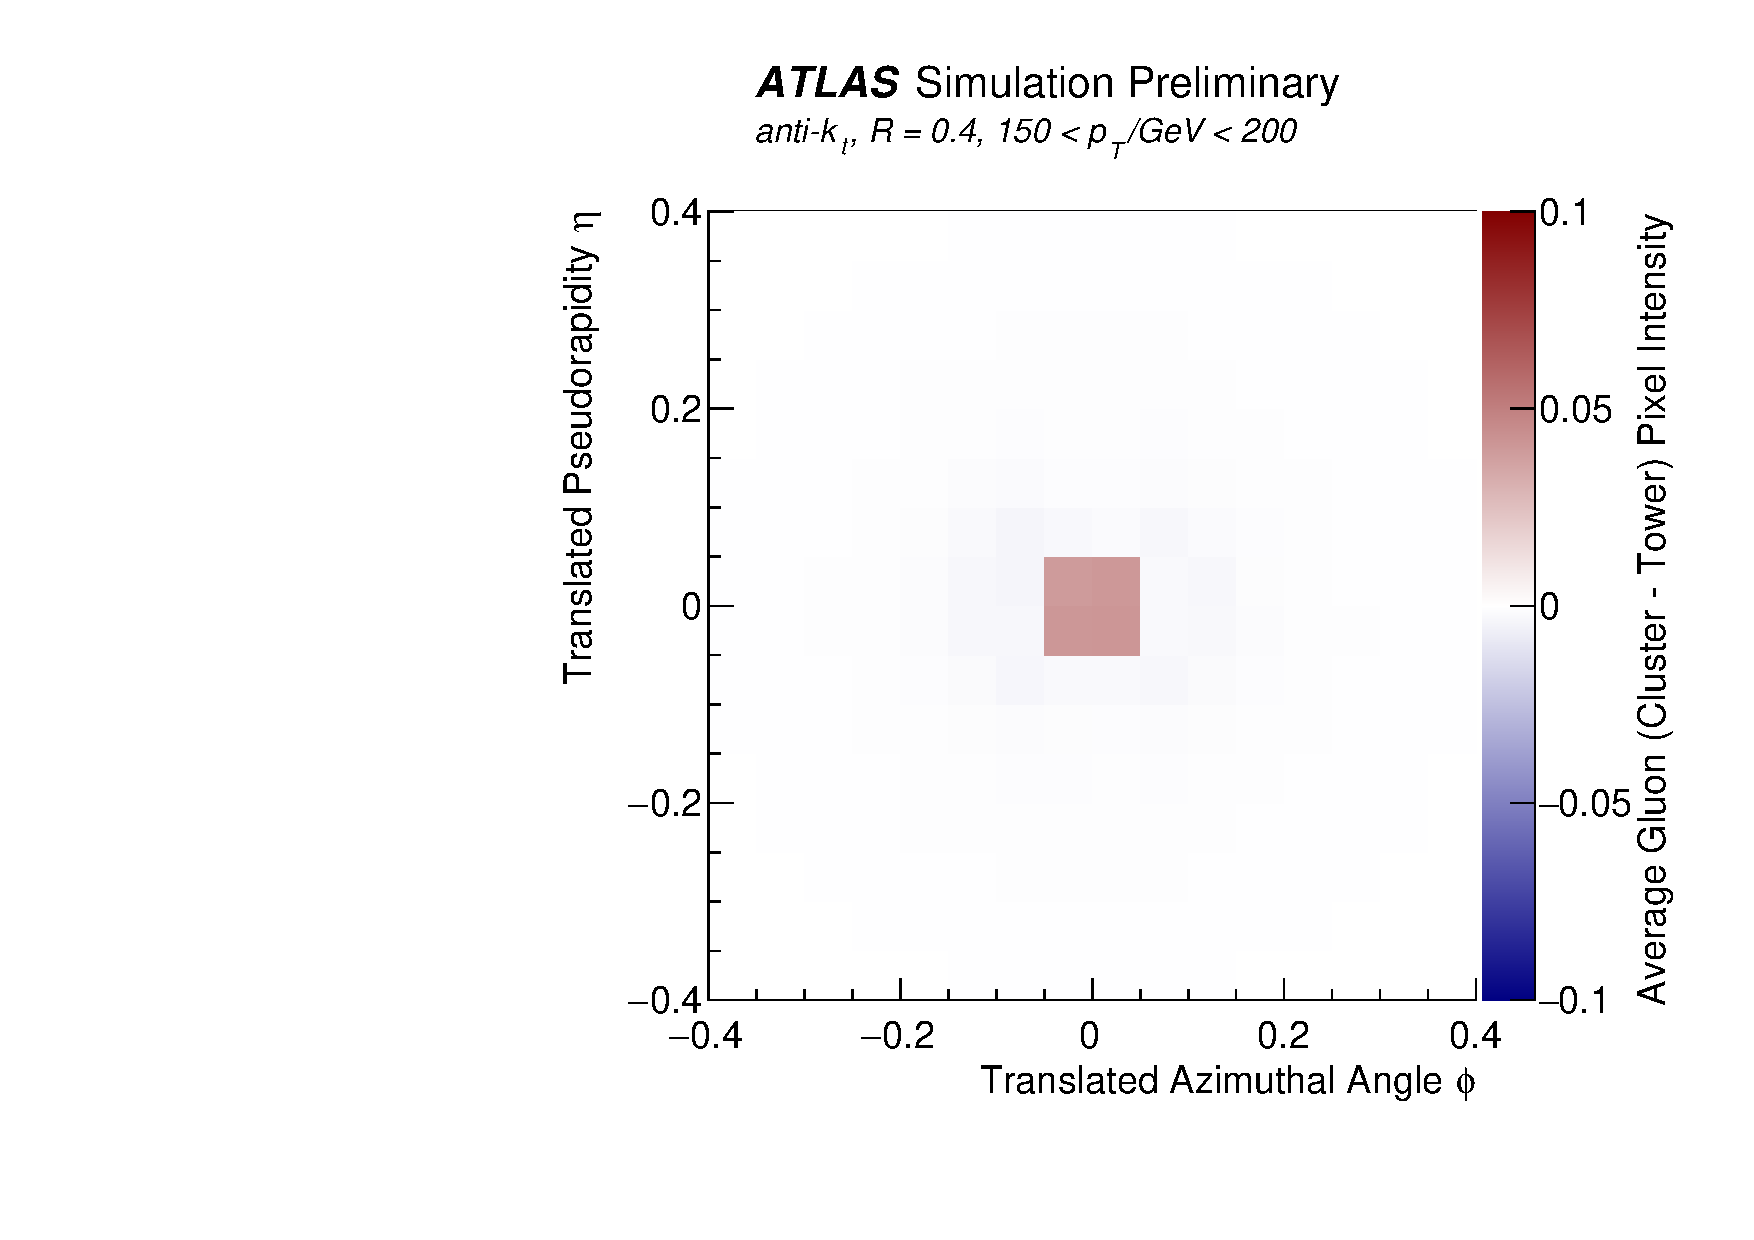
\includegraphics[width=0.31\textwidth]{figures/CNN/diff_gluon_cluster_tower.pdf}
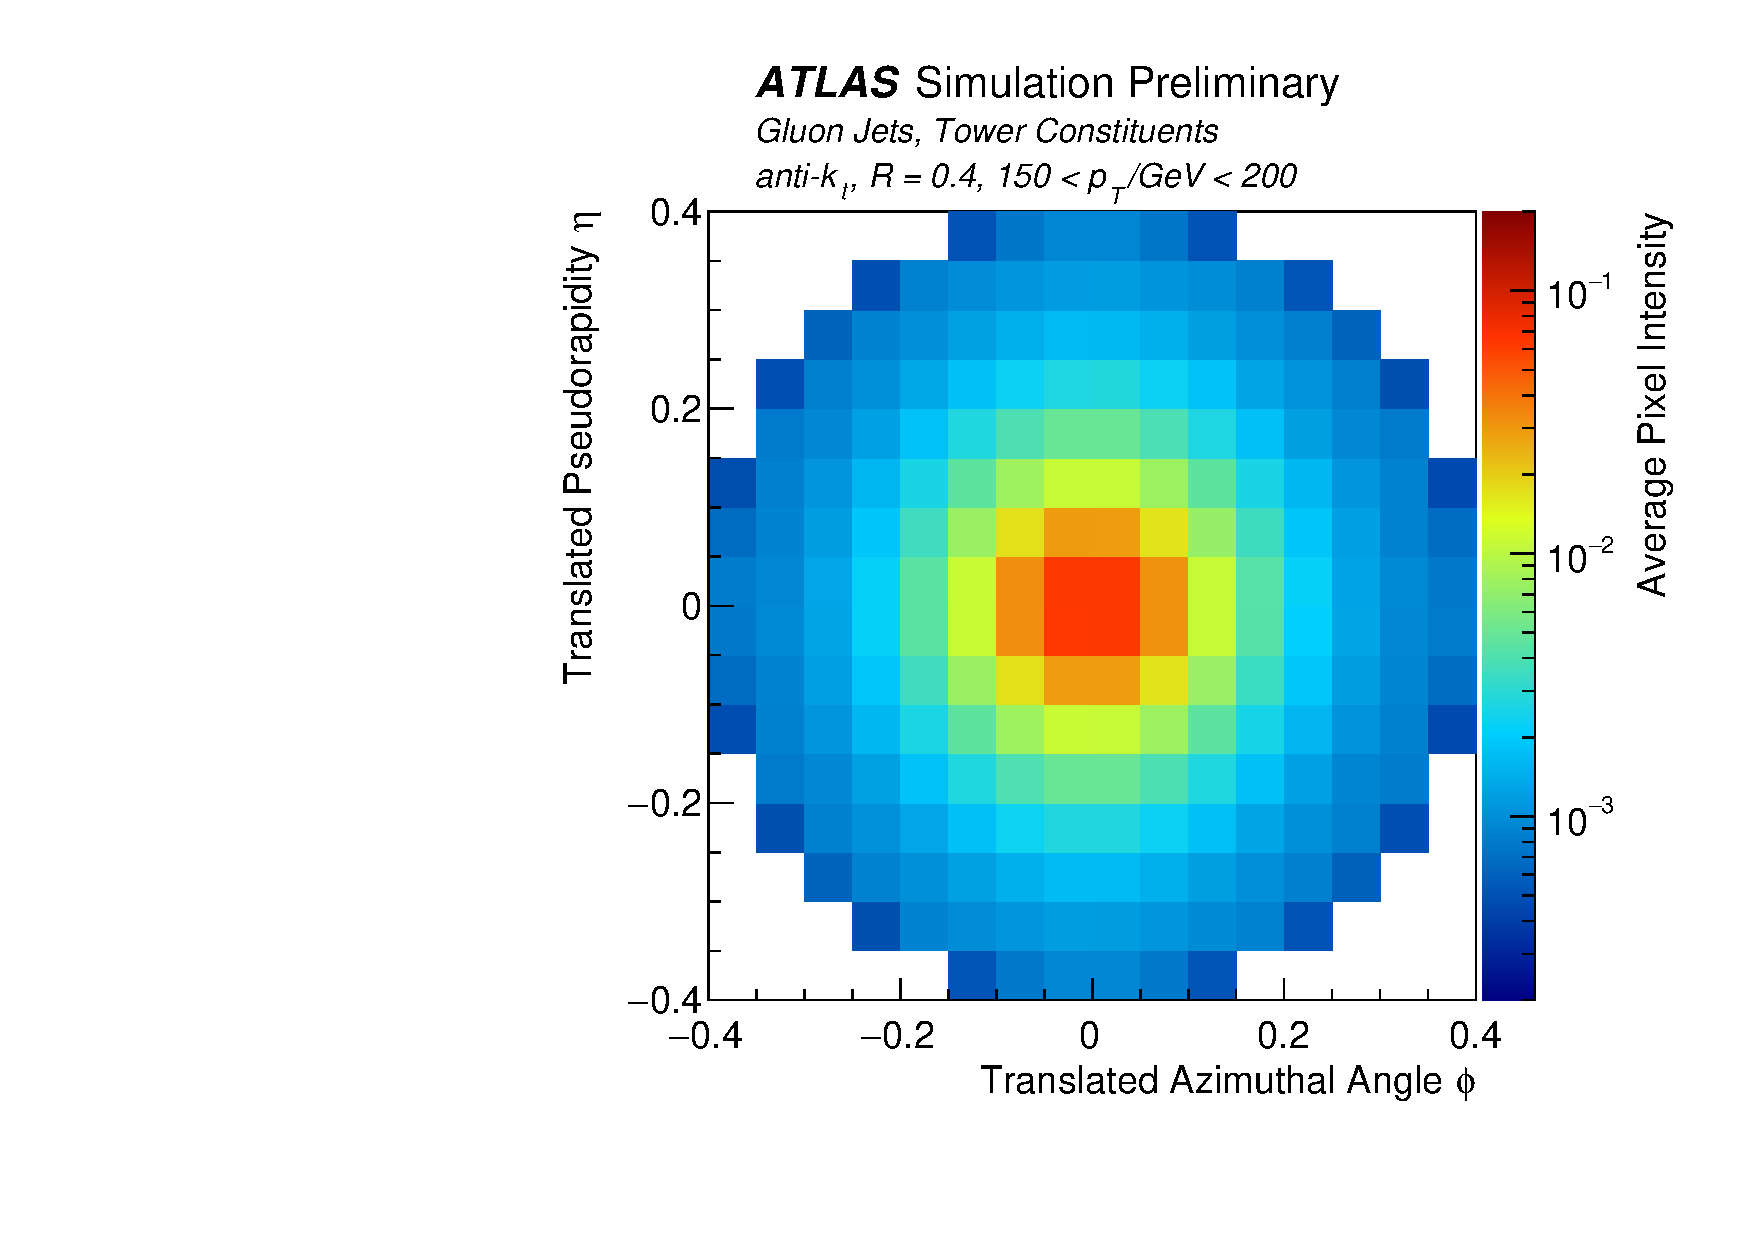
\includegraphics[width=0.31\textwidth]{figures/CNN/gluon_tower.pdf}
\caption{The four corners show the average quark (upper) and gluon (lower) jet images, from topo-clusters (left) and towers (right); the four plots on the edges show the difference between the adjacent plots, for example the top plot shows the difference between the average quark jet for topoclusters and towers. Quark-jets are more collimated than gluon ones, and topo-cluster images are more collimated than tower images.}
\label{fig:cnn-avg:clustertower}
\end{center}
\end{figure}

\clearpage

